\documentclass[twoside]{book}

% Packages required by doxygen
\usepackage{fixltx2e}
\usepackage{calc}
\usepackage{doxygen}
\usepackage[export]{adjustbox} % also loads graphicx
\usepackage{graphicx}
\usepackage[utf8]{inputenc}
\usepackage{makeidx}
\usepackage{multicol}
\usepackage{multirow}
\PassOptionsToPackage{warn}{textcomp}
\usepackage{textcomp}
\usepackage[nointegrals]{wasysym}
\usepackage[table]{xcolor}

% Font selection
\usepackage[T1]{fontenc}
\usepackage[scaled=.90]{helvet}
\usepackage{courier}
\usepackage{amssymb}
\usepackage{sectsty}
\renewcommand{\familydefault}{\sfdefault}
\allsectionsfont{%
  \fontseries{bc}\selectfont%
  \color{darkgray}%
}
\renewcommand{\DoxyLabelFont}{%
  \fontseries{bc}\selectfont%
  \color{darkgray}%
}
\newcommand{\+}{\discretionary{\mbox{\scriptsize$\hookleftarrow$}}{}{}}

% Page & text layout
\usepackage{geometry}
\geometry{%
  a4paper,%
  top=2.5cm,%
  bottom=2.5cm,%
  left=2.5cm,%
  right=2.5cm%
}
\tolerance=750
\hfuzz=15pt
\hbadness=750
\setlength{\emergencystretch}{15pt}
\setlength{\parindent}{0cm}
\setlength{\parskip}{0.2cm}
\makeatletter
\renewcommand{\paragraph}{%
  \@startsection{paragraph}{4}{0ex}{-1.0ex}{1.0ex}{%
    \normalfont\normalsize\bfseries\SS@parafont%
  }%
}
\renewcommand{\subparagraph}{%
  \@startsection{subparagraph}{5}{0ex}{-1.0ex}{1.0ex}{%
    \normalfont\normalsize\bfseries\SS@subparafont%
  }%
}
\makeatother

% Headers & footers
\usepackage{fancyhdr}
\pagestyle{fancyplain}
\fancyhead[LE]{\fancyplain{}{\bfseries\thepage}}
\fancyhead[CE]{\fancyplain{}{}}
\fancyhead[RE]{\fancyplain{}{\bfseries\leftmark}}
\fancyhead[LO]{\fancyplain{}{\bfseries\rightmark}}
\fancyhead[CO]{\fancyplain{}{}}
\fancyhead[RO]{\fancyplain{}{\bfseries\thepage}}
\fancyfoot[LE]{\fancyplain{}{}}
\fancyfoot[CE]{\fancyplain{}{}}
\fancyfoot[RE]{\fancyplain{}{\bfseries\scriptsize Generated on Thu Mar 31 2016 07\+:14\+:37 for Cross-\/and-\/circle-\/game by Doxygen }}
\fancyfoot[LO]{\fancyplain{}{\bfseries\scriptsize Generated on Thu Mar 31 2016 07\+:14\+:37 for Cross-\/and-\/circle-\/game by Doxygen }}
\fancyfoot[CO]{\fancyplain{}{}}
\fancyfoot[RO]{\fancyplain{}{}}
\renewcommand{\footrulewidth}{0.4pt}
\renewcommand{\chaptermark}[1]{%
  \markboth{#1}{}%
}
\renewcommand{\sectionmark}[1]{%
  \markright{\thesection\ #1}%
}

% Indices & bibliography
\usepackage{natbib}
\usepackage[titles]{tocloft}
\setcounter{tocdepth}{3}
\setcounter{secnumdepth}{5}
\makeindex

% Hyperlinks (required, but should be loaded last)
\usepackage{ifpdf}
\ifpdf
  \usepackage[pdftex,pagebackref=true]{hyperref}
\else
  \usepackage[ps2pdf,pagebackref=true]{hyperref}
\fi
\hypersetup{%
  colorlinks=true,%
  linkcolor=blue,%
  citecolor=blue,%
  unicode%
}

% Custom commands
\newcommand{\clearemptydoublepage}{%
  \newpage{\pagestyle{empty}\cleardoublepage}%
}


%===== C O N T E N T S =====

\begin{document}

% Titlepage & ToC
\hypersetup{pageanchor=false,
             bookmarks=true,
             bookmarksnumbered=true,
             pdfencoding=unicode
            }
\pagenumbering{roman}
\begin{titlepage}
\vspace*{7cm}
\begin{center}%
{\Large Cross-\/and-\/circle-\/game \\[1ex]\large 0.\+02 }\\
\vspace*{1cm}
{\large Generated by Doxygen 1.8.9.1}\\
\vspace*{0.5cm}
{\small Thu Mar 31 2016 07:14:37}\\
\end{center}
\end{titlepage}
\clearemptydoublepage
\tableofcontents
\clearemptydoublepage
\pagenumbering{arabic}
\hypersetup{pageanchor=true}

%--- Begin generated contents ---
\chapter{Main Page}
\label{index}\hypertarget{index}{}Simple game.\begin{DoxyNote}{Note}
with gh-\/pages
\end{DoxyNote}
\begin{DoxyAuthor}{Author}
Fotoblysk
\end{DoxyAuthor}
\begin{DoxyVersion}{Version}

\end{DoxyVersion}
\begin{DoxyParagraph}{Revision}
0.\+01 
\end{DoxyParagraph}


\begin{DoxyDate}{Date}
2016/03/13 21\+:44\+:00
\end{DoxyDate}
Contact\+: \href{mailto:fotoblysk@fejm.pl}{\tt fotoblysk@fejm.\+pl}

Created on\+: Sun Mar 13 21\+:44\+:00 2016

\begin{DoxyParagraph}{Id}
Cross-\/and-\/circle-\/game,v 0.\+01 21\+:44\+:00 bv Exp Fotoblysk
\end{DoxyParagraph}

\chapter{Cross-\/and-\/circle-\/game}
\label{md__c_1__users__foto__documents__git_hub__cross-and-circle-game__r_e_a_d_m_e}
\hypertarget{md__c_1__users__foto__documents__git_hub__cross-and-circle-game__r_e_a_d_m_e}{}
Cross and circle game c++ using S\+F\+M\+L-\/2.\+3.\+2 
\chapter{Hierarchical Index}
\section{Class Hierarchy}
This inheritance list is sorted roughly, but not completely, alphabetically\+:\begin{DoxyCompactList}
\item \contentsline{section}{lol}{\pageref{classlol}}{}
\begin{DoxyCompactList}
\item \contentsline{section}{xd}{\pageref{classxd}}{}
\end{DoxyCompactList}
\end{DoxyCompactList}

\chapter{Class Index}
\section{Class List}
Here are the classes, structs, unions and interfaces with brief descriptions\+:\begin{DoxyCompactList}
\item\contentsline{section}{\hyperlink{class_board}{Board} \\*\hyperlink{class_engine}{Engine} class. Class which manage main loop of game, reads keyboard events, update physics. This class will menage menu and settings }{\pageref{class_board}}{}
\item\contentsline{section}{\hyperlink{class_engine_1_1cpp}{Engine\+::cpp} }{\pageref{class_engine_1_1cpp}}{}
\item\contentsline{section}{\hyperlink{class_engine}{Engine} \\*\hyperlink{class_engine}{Engine} class. Class which manage main loop of game, reads keyboard events, update physics. This class will menage menu and settings }{\pageref{class_engine}}{}
\item\contentsline{section}{\hyperlink{class_game}{Game} \\*\hyperlink{class_game}{Game} main class. Class which is used run engine. This class will menage menu and settings }{\pageref{class_game}}{}
\item\contentsline{section}{\hyperlink{class_player}{Player} \\*\hyperlink{class_player}{Player} class -\/ pointers to player have a lot of usage in program. All Squares have pointer to player which were marked by pointers to players are also used by \hyperlink{class_engine}{Engine} class to set whose turn is now }{\pageref{class_player}}{}
\item\contentsline{section}{\hyperlink{class_square}{Square} \\*\hyperlink{class_square}{Square} class. Class which is used to build board this class may be remade to inheritance from sf\+::\+Rectangle\+Shape }{\pageref{class_square}}{}
\end{DoxyCompactList}

\chapter{File Index}
\section{File List}
Here is a list of all documented files with brief descriptions\+:\begin{DoxyCompactList}
\item\contentsline{section}{\hyperlink{main_8cpp}{main.\+cpp} \\*Main file of the program }{\pageref{main_8cpp}}{}
\end{DoxyCompactList}

\chapter{Class Documentation}
\hypertarget{class_board}{}\section{Board Class Reference}
\label{class_board}\index{Board@{Board}}


\hyperlink{class_engine}{Engine} class. Class which manage main loop of game, reads keyboard events, update physics. This class will menage menu and settings.  




{\ttfamily \#include $<$Board.\+h$>$}



Inheritance diagram for Board\+:
\nopagebreak
\begin{figure}[H]
\begin{center}
\leavevmode
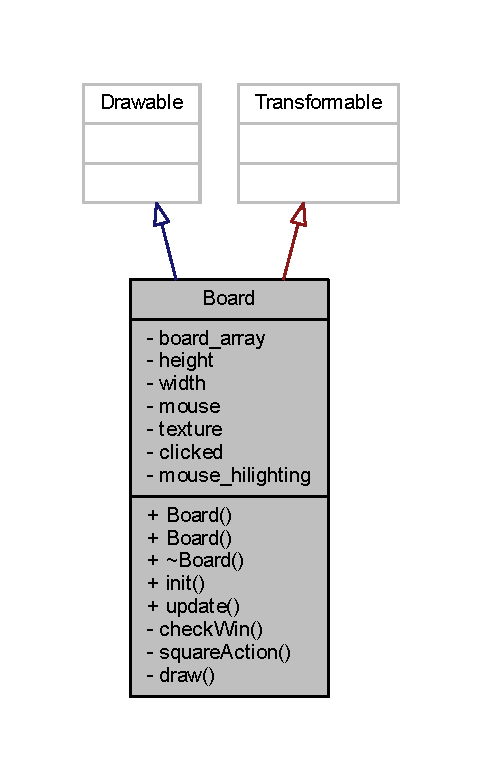
\includegraphics[width=232pt]{class_board__inherit__graph}
\end{center}
\end{figure}


Collaboration diagram for Board\+:
\nopagebreak
\begin{figure}[H]
\begin{center}
\leavevmode
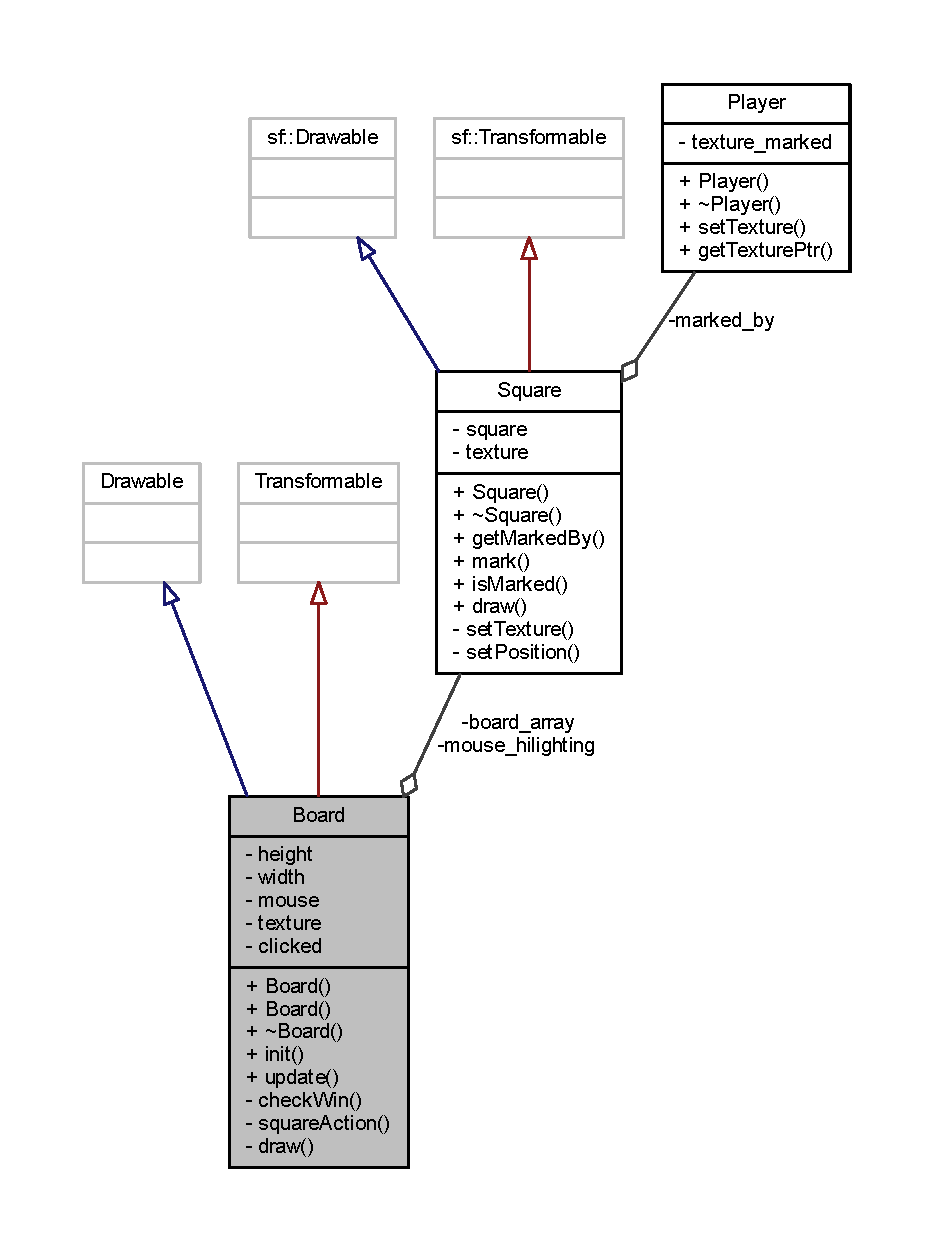
\includegraphics[width=350pt]{class_board__coll__graph}
\end{center}
\end{figure}
\subsection*{Public Member Functions}
\begin{DoxyCompactItemize}
\item 
\hyperlink{class_board_a9ee491d4fea680cf69b033374a9fdfcb}{Board} ()
\begin{DoxyCompactList}\small\item\em pointers to null . vars to 0. \hyperlink{class_board}{Board} useless until initialized with init(...) \end{DoxyCompactList}\item 
\hyperlink{class_board_af98d75fee5ec0d1fc87a41a64a2dea91}{Board} (int height\+\_\+in, int width\+\_\+in, sf\+::\+Vector2i $\ast$mouse\+\_\+in)
\begin{DoxyCompactList}\small\item\em inits board sets size and mouse var allocates dynamic array of squares (runs init function). \end{DoxyCompactList}\item 
virtual \hyperlink{class_board_af73f45730119a1fd8f6670f53f959e68}{$\sim$\+Board} ()
\item 
void \hyperlink{class_board_a7bb620341249cac1e5366e4fe0c91135}{init} (int height\+\_\+in, int width\+\_\+in, sf\+::\+Vector2i $\ast$mouse\+\_\+in)
\begin{DoxyCompactList}\small\item\em inits board sets size and mouse var \end{DoxyCompactList}\item 
bool \hyperlink{class_board_a05f30f65527fdbfe4950040f2e44da6f}{update} (bool $\ast$marked\+\_\+in, \hyperlink{class_player}{Player} $\ast$$\ast$currrent\+\_\+turn)
\begin{DoxyCompactList}\small\item\em updates board highlight squares (pointlesss setting Player$\ast$$\ast$ doing in evry loop -\/ move to init)-\/ pointer remember pointer ids pointing to. \end{DoxyCompactList}\end{DoxyCompactItemize}
\subsection*{Private Member Functions}
\begin{DoxyCompactItemize}
\item 
bool \hyperlink{class_board_a4f79d2766626e4167c2b65a43f051545}{check\+Win} (int height\+\_\+index, int width\+\_\+index, \hyperlink{class_player}{Player} $\ast$$\ast$current\+\_\+turn)
\item 
bool \hyperlink{class_board_a204e367441e2b61d02721e70fb0b9a99}{square\+Action} (int height\+\_\+index, int width\+\_\+index, \hyperlink{class_player}{Player} $\ast$$\ast$currrent\+\_\+turn)
\begin{DoxyCompactList}\small\item\em checks if just done turn have made current player winnner \end{DoxyCompactList}\item 
virtual void \hyperlink{class_board_a92d6dbe56e7fc7e96633c80a505a12b3}{draw} (sf\+::\+Render\+Target \&target, sf\+::\+Render\+States states) const 
\begin{DoxyCompactList}\small\item\em draws all squares. this is used after all seting what to hilight, mark, ect \end{DoxyCompactList}\end{DoxyCompactItemize}
\subsection*{Private Attributes}
\begin{DoxyCompactItemize}
\item 
\hyperlink{class_square}{Square} $\ast$$\ast$ \hyperlink{class_board_aae4209ee856592868709d92081368777}{board\+\_\+array}
\begin{DoxyCompactList}\small\item\em pointer to dynamic allocated array of squares. deletes in destructor \end{DoxyCompactList}\item 
int \hyperlink{class_board_aa0cb8de0254520dc08dab5796643c8e5}{height}
\begin{DoxyCompactList}\small\item\em height of the dynamic array of squares \end{DoxyCompactList}\item 
int \hyperlink{class_board_a90a8efaa4736af25511ac948bdd27d6c}{width}
\begin{DoxyCompactList}\small\item\em width of the dynamic array of squares \end{DoxyCompactList}\item 
sf\+::\+Vector2i $\ast$ \hyperlink{class_board_a70eb26b4e2928c9eb58f9072380ced54}{mouse}
\begin{DoxyCompactList}\small\item\em pointer to mouse var from \hyperlink{class_engine}{Engine} \end{DoxyCompactList}\item 
sf\+::\+Texture \hyperlink{class_board_a34d04abd4e0c5212e5a32cdd39263298}{texture}
\begin{DoxyCompactList}\small\item\em basic evry single square texture \end{DoxyCompactList}\item 
bool $\ast$ \hyperlink{class_board_adbf08097362eabd4621b777261c2e4d7}{clicked}
\begin{DoxyCompactList}\small\item\em pointer to var witch says if \end{DoxyCompactList}\item 
\hyperlink{class_square}{Square} $\ast$ \hyperlink{class_board_a27c871bcf6b8eb8bb8af2f28a4c7a909}{mouse\+\_\+hilighting}
\begin{DoxyCompactList}\small\item\em pointer to square on which mouse is on highlight \end{DoxyCompactList}\end{DoxyCompactItemize}


\subsection{Detailed Description}
\hyperlink{class_engine}{Engine} class. Class which manage main loop of game, reads keyboard events, update physics. This class will menage menu and settings. 

\subsection{Constructor \& Destructor Documentation}
\hypertarget{class_board_a9ee491d4fea680cf69b033374a9fdfcb}{}\index{Board@{Board}!Board@{Board}}
\index{Board@{Board}!Board@{Board}}
\subsubsection[{Board}]{\setlength{\rightskip}{0pt plus 5cm}Board\+::\+Board (
\begin{DoxyParamCaption}
{}
\end{DoxyParamCaption}
)}\label{class_board_a9ee491d4fea680cf69b033374a9fdfcb}


pointers to null . vars to 0. \hyperlink{class_board}{Board} useless until initialized with init(...) 

\hypertarget{class_board_af98d75fee5ec0d1fc87a41a64a2dea91}{}\index{Board@{Board}!Board@{Board}}
\index{Board@{Board}!Board@{Board}}
\subsubsection[{Board}]{\setlength{\rightskip}{0pt plus 5cm}Board\+::\+Board (
\begin{DoxyParamCaption}
\item[{int}]{height\+\_\+in, }
\item[{int}]{width\+\_\+in, }
\item[{sf\+::\+Vector2i $\ast$}]{mouse\+\_\+in}
\end{DoxyParamCaption}
)}\label{class_board_af98d75fee5ec0d1fc87a41a64a2dea91}


inits board sets size and mouse var allocates dynamic array of squares (runs init function). 



Here is the call graph for this function\+:\nopagebreak
\begin{figure}[H]
\begin{center}
\leavevmode
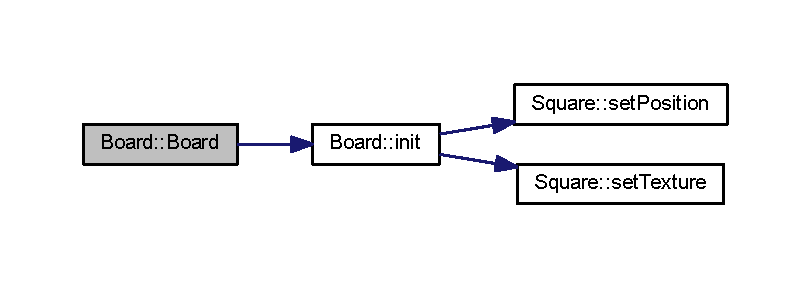
\includegraphics[width=350pt]{class_board_af98d75fee5ec0d1fc87a41a64a2dea91_cgraph}
\end{center}
\end{figure}


\hypertarget{class_board_af73f45730119a1fd8f6670f53f959e68}{}\index{Board@{Board}!````~Board@{$\sim$\+Board}}
\index{````~Board@{$\sim$\+Board}!Board@{Board}}
\subsubsection[{$\sim$\+Board}]{\setlength{\rightskip}{0pt plus 5cm}Board\+::$\sim$\+Board (
\begin{DoxyParamCaption}
{}
\end{DoxyParamCaption}
)\hspace{0.3cm}{\ttfamily [virtual]}}\label{class_board_af73f45730119a1fd8f6670f53f959e68}


\subsection{Member Function Documentation}
\hypertarget{class_board_a4f79d2766626e4167c2b65a43f051545}{}\index{Board@{Board}!check\+Win@{check\+Win}}
\index{check\+Win@{check\+Win}!Board@{Board}}
\subsubsection[{check\+Win}]{\setlength{\rightskip}{0pt plus 5cm}bool Board\+::check\+Win (
\begin{DoxyParamCaption}
\item[{int}]{height\+\_\+index, }
\item[{int}]{width\+\_\+index, }
\item[{{\bf Player} $\ast$$\ast$}]{current\+\_\+turn}
\end{DoxyParamCaption}
)\hspace{0.3cm}{\ttfamily [private]}}\label{class_board_a4f79d2766626e4167c2b65a43f051545}


Here is the caller graph for this function\+:\nopagebreak
\begin{figure}[H]
\begin{center}
\leavevmode
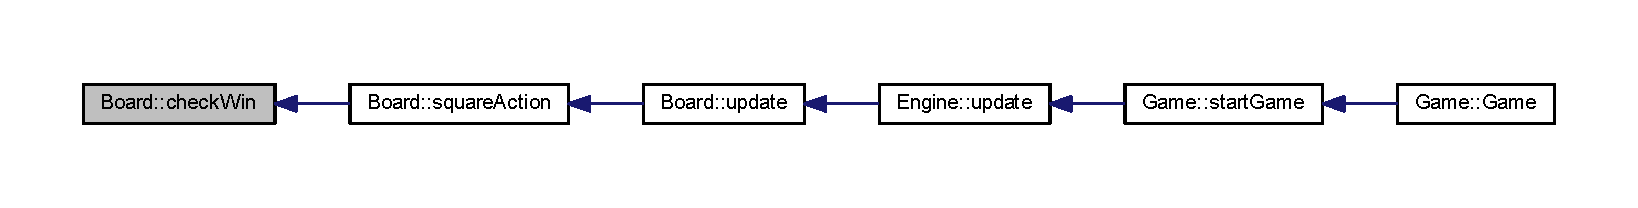
\includegraphics[width=350pt]{class_board_a4f79d2766626e4167c2b65a43f051545_icgraph}
\end{center}
\end{figure}


\hypertarget{class_board_a92d6dbe56e7fc7e96633c80a505a12b3}{}\index{Board@{Board}!draw@{draw}}
\index{draw@{draw}!Board@{Board}}
\subsubsection[{draw}]{\setlength{\rightskip}{0pt plus 5cm}void Board\+::draw (
\begin{DoxyParamCaption}
\item[{sf\+::\+Render\+Target \&}]{target, }
\item[{sf\+::\+Render\+States}]{states}
\end{DoxyParamCaption}
) const\hspace{0.3cm}{\ttfamily [private]}, {\ttfamily [virtual]}}\label{class_board_a92d6dbe56e7fc7e96633c80a505a12b3}


draws all squares. this is used after all seting what to hilight, mark, ect 

\hypertarget{class_board_a7bb620341249cac1e5366e4fe0c91135}{}\index{Board@{Board}!init@{init}}
\index{init@{init}!Board@{Board}}
\subsubsection[{init}]{\setlength{\rightskip}{0pt plus 5cm}void Board\+::init (
\begin{DoxyParamCaption}
\item[{int}]{height\+\_\+in, }
\item[{int}]{width\+\_\+in, }
\item[{sf\+::\+Vector2i $\ast$}]{mouse\+\_\+in}
\end{DoxyParamCaption}
)}\label{class_board_a7bb620341249cac1e5366e4fe0c91135}


inits board sets size and mouse var 



Here is the call graph for this function\+:\nopagebreak
\begin{figure}[H]
\begin{center}
\leavevmode
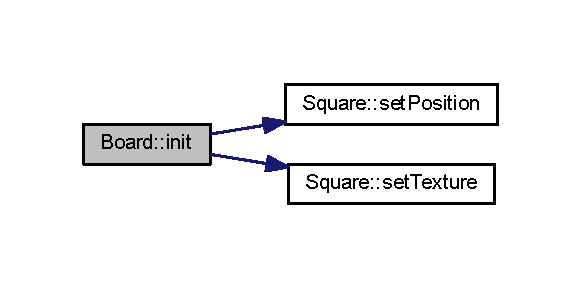
\includegraphics[width=279pt]{class_board_a7bb620341249cac1e5366e4fe0c91135_cgraph}
\end{center}
\end{figure}




Here is the caller graph for this function\+:\nopagebreak
\begin{figure}[H]
\begin{center}
\leavevmode
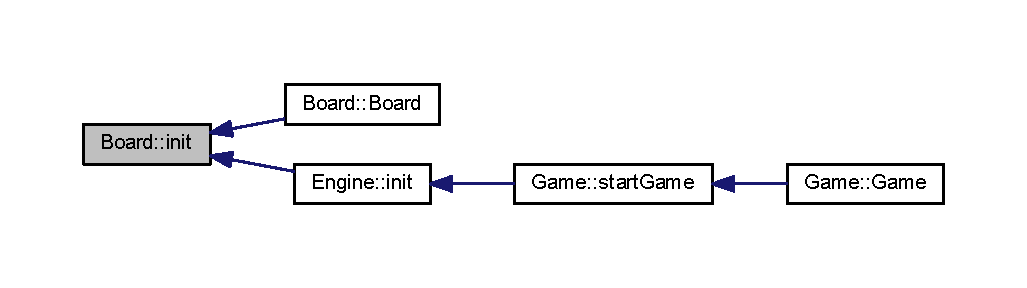
\includegraphics[width=350pt]{class_board_a7bb620341249cac1e5366e4fe0c91135_icgraph}
\end{center}
\end{figure}


\hypertarget{class_board_a204e367441e2b61d02721e70fb0b9a99}{}\index{Board@{Board}!square\+Action@{square\+Action}}
\index{square\+Action@{square\+Action}!Board@{Board}}
\subsubsection[{square\+Action}]{\setlength{\rightskip}{0pt plus 5cm}bool Board\+::square\+Action (
\begin{DoxyParamCaption}
\item[{int}]{height\+\_\+index, }
\item[{int}]{width\+\_\+index, }
\item[{{\bf Player} $\ast$$\ast$}]{currrent\+\_\+turn}
\end{DoxyParamCaption}
)\hspace{0.3cm}{\ttfamily [private]}}\label{class_board_a204e367441e2b61d02721e70fb0b9a99}


checks if just done turn have made current player winnner 

action of single square Player$\ast$$\ast$ is a pointer to current players turn from \hyperlink{class_engine}{Engine} class !!!! Tododododo have to fix that 

Here is the call graph for this function\+:
\nopagebreak
\begin{figure}[H]
\begin{center}
\leavevmode
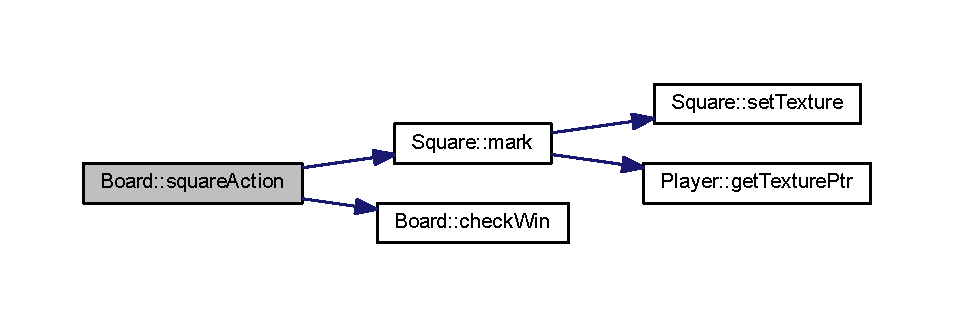
\includegraphics[width=350pt]{class_board_a204e367441e2b61d02721e70fb0b9a99_cgraph}
\end{center}
\end{figure}




Here is the caller graph for this function\+:\nopagebreak
\begin{figure}[H]
\begin{center}
\leavevmode
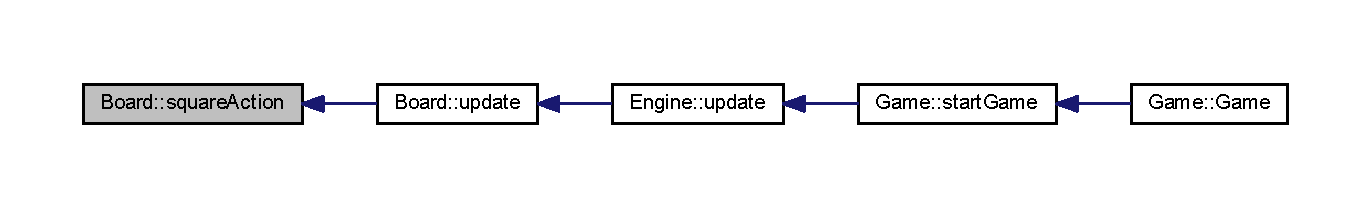
\includegraphics[width=350pt]{class_board_a204e367441e2b61d02721e70fb0b9a99_icgraph}
\end{center}
\end{figure}


\hypertarget{class_board_a05f30f65527fdbfe4950040f2e44da6f}{}\index{Board@{Board}!update@{update}}
\index{update@{update}!Board@{Board}}
\subsubsection[{update}]{\setlength{\rightskip}{0pt plus 5cm}bool Board\+::update (
\begin{DoxyParamCaption}
\item[{bool $\ast$}]{marked\+\_\+in, }
\item[{{\bf Player} $\ast$$\ast$}]{currrent\+\_\+turn}
\end{DoxyParamCaption}
)}\label{class_board_a05f30f65527fdbfe4950040f2e44da6f}


updates board highlight squares (pointlesss setting Player$\ast$$\ast$ doing in evry loop -\/ move to init)-\/ pointer remember pointer ids pointing to. 



Here is the call graph for this function\+:
\nopagebreak
\begin{figure}[H]
\begin{center}
\leavevmode
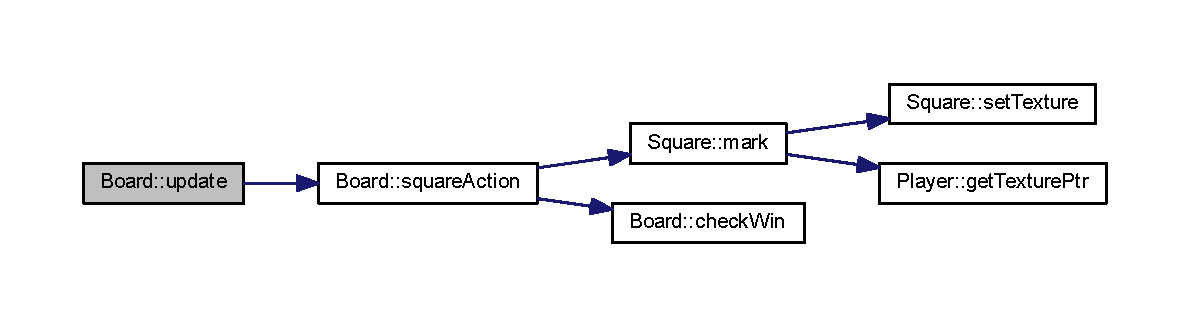
\includegraphics[width=350pt]{class_board_a05f30f65527fdbfe4950040f2e44da6f_cgraph}
\end{center}
\end{figure}




Here is the caller graph for this function\+:\nopagebreak
\begin{figure}[H]
\begin{center}
\leavevmode
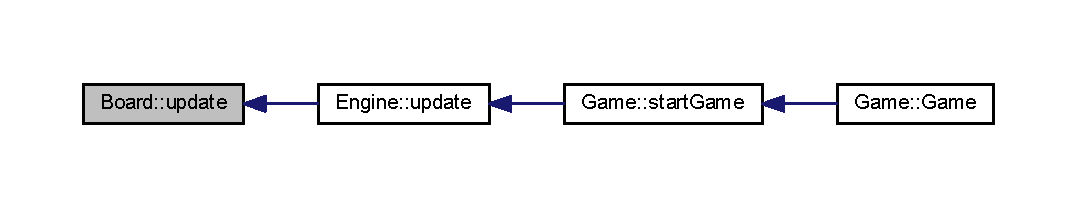
\includegraphics[width=350pt]{class_board_a05f30f65527fdbfe4950040f2e44da6f_icgraph}
\end{center}
\end{figure}




\subsection{Member Data Documentation}
\hypertarget{class_board_aae4209ee856592868709d92081368777}{}\index{Board@{Board}!board\+\_\+array@{board\+\_\+array}}
\index{board\+\_\+array@{board\+\_\+array}!Board@{Board}}
\subsubsection[{board\+\_\+array}]{\setlength{\rightskip}{0pt plus 5cm}{\bf Square}$\ast$$\ast$ Board\+::board\+\_\+array\hspace{0.3cm}{\ttfamily [private]}}\label{class_board_aae4209ee856592868709d92081368777}


pointer to dynamic allocated array of squares. deletes in destructor 

\hypertarget{class_board_adbf08097362eabd4621b777261c2e4d7}{}\index{Board@{Board}!clicked@{clicked}}
\index{clicked@{clicked}!Board@{Board}}
\subsubsection[{clicked}]{\setlength{\rightskip}{0pt plus 5cm}bool$\ast$ Board\+::clicked\hspace{0.3cm}{\ttfamily [private]}}\label{class_board_adbf08097362eabd4621b777261c2e4d7}


pointer to var witch says if 

\hypertarget{class_board_aa0cb8de0254520dc08dab5796643c8e5}{}\index{Board@{Board}!height@{height}}
\index{height@{height}!Board@{Board}}
\subsubsection[{height}]{\setlength{\rightskip}{0pt plus 5cm}int Board\+::height\hspace{0.3cm}{\ttfamily [private]}}\label{class_board_aa0cb8de0254520dc08dab5796643c8e5}


height of the dynamic array of squares 

\hypertarget{class_board_a70eb26b4e2928c9eb58f9072380ced54}{}\index{Board@{Board}!mouse@{mouse}}
\index{mouse@{mouse}!Board@{Board}}
\subsubsection[{mouse}]{\setlength{\rightskip}{0pt plus 5cm}sf\+::\+Vector2i$\ast$ Board\+::mouse\hspace{0.3cm}{\ttfamily [private]}}\label{class_board_a70eb26b4e2928c9eb58f9072380ced54}


pointer to mouse var from \hyperlink{class_engine}{Engine} 

\hypertarget{class_board_a27c871bcf6b8eb8bb8af2f28a4c7a909}{}\index{Board@{Board}!mouse\+\_\+hilighting@{mouse\+\_\+hilighting}}
\index{mouse\+\_\+hilighting@{mouse\+\_\+hilighting}!Board@{Board}}
\subsubsection[{mouse\+\_\+hilighting}]{\setlength{\rightskip}{0pt plus 5cm}{\bf Square}$\ast$ Board\+::mouse\+\_\+hilighting\hspace{0.3cm}{\ttfamily [private]}}\label{class_board_a27c871bcf6b8eb8bb8af2f28a4c7a909}


pointer to square on which mouse is on highlight 

\hypertarget{class_board_a34d04abd4e0c5212e5a32cdd39263298}{}\index{Board@{Board}!texture@{texture}}
\index{texture@{texture}!Board@{Board}}
\subsubsection[{texture}]{\setlength{\rightskip}{0pt plus 5cm}sf\+::\+Texture Board\+::texture\hspace{0.3cm}{\ttfamily [private]}}\label{class_board_a34d04abd4e0c5212e5a32cdd39263298}


basic evry single square texture 

\hypertarget{class_board_a90a8efaa4736af25511ac948bdd27d6c}{}\index{Board@{Board}!width@{width}}
\index{width@{width}!Board@{Board}}
\subsubsection[{width}]{\setlength{\rightskip}{0pt plus 5cm}int Board\+::width\hspace{0.3cm}{\ttfamily [private]}}\label{class_board_a90a8efaa4736af25511ac948bdd27d6c}


width of the dynamic array of squares 



The documentation for this class was generated from the following files\+:\begin{DoxyCompactItemize}
\item 
\hyperlink{_board_8h}{Board.\+h}\item 
\hyperlink{_board_8cpp}{Board.\+cpp}\end{DoxyCompactItemize}

\hypertarget{class_engine_1_1cpp}{}\section{Engine\+:\+:cpp Class Reference}
\label{class_engine_1_1cpp}\index{Engine\+::cpp@{Engine\+::cpp}}


{\ttfamily \#include $<$Engine.\+cpp.\+h$>$}



Collaboration diagram for Engine\+:\+:cpp\+:\nopagebreak
\begin{figure}[H]
\begin{center}
\leavevmode
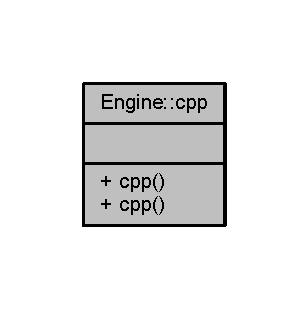
\includegraphics[width=148pt]{class_engine_1_1cpp__coll__graph}
\end{center}
\end{figure}
\subsection*{Public Member Functions}
\begin{DoxyCompactItemize}
\item 
\hyperlink{class_engine}{Engine} \hyperlink{class_engine_1_1cpp_ac11d32b481cab653cb32e82b4007976f}{cpp} ()
\item 
virtual $\sim$\hyperlink{class_engine}{Engine} \hyperlink{class_engine_1_1cpp_ad08768b0f971619c7917a24438509162}{cpp} ()
\end{DoxyCompactItemize}


\subsection{Constructor \& Destructor Documentation}
\hypertarget{class_engine_1_1cpp_ac11d32b481cab653cb32e82b4007976f}{}\index{Engine\+::cpp@{Engine\+::cpp}!cpp@{cpp}}
\index{cpp@{cpp}!Engine\+::cpp@{Engine\+::cpp}}
\subsubsection[{cpp}]{\setlength{\rightskip}{0pt plus 5cm}{\bf Engine} Engine\+::cpp\+::cpp (
\begin{DoxyParamCaption}
{}
\end{DoxyParamCaption}
)}\label{class_engine_1_1cpp_ac11d32b481cab653cb32e82b4007976f}
\hypertarget{class_engine_1_1cpp_ad08768b0f971619c7917a24438509162}{}\index{Engine\+::cpp@{Engine\+::cpp}!cpp@{cpp}}
\index{cpp@{cpp}!Engine\+::cpp@{Engine\+::cpp}}
\subsubsection[{cpp}]{\setlength{\rightskip}{0pt plus 5cm}virtual $\sim${\bf Engine} Engine\+::cpp\+::cpp (
\begin{DoxyParamCaption}
{}
\end{DoxyParamCaption}
)\hspace{0.3cm}{\ttfamily [virtual]}}\label{class_engine_1_1cpp_ad08768b0f971619c7917a24438509162}


The documentation for this class was generated from the following file\+:\begin{DoxyCompactItemize}
\item 
\hyperlink{_engine_8cpp_8h}{Engine.\+cpp.\+h}\end{DoxyCompactItemize}

\hypertarget{class_engine}{}\section{Engine Class Reference}
\label{class_engine}\index{Engine@{Engine}}


\hyperlink{class_engine}{Engine} class. Class which manage main loop of game, reads keyboard events, update physics. This class will menage menu and settings.  




{\ttfamily \#include $<$Engine.\+h$>$}



Collaboration diagram for Engine\+:
\nopagebreak
\begin{figure}[H]
\begin{center}
\leavevmode
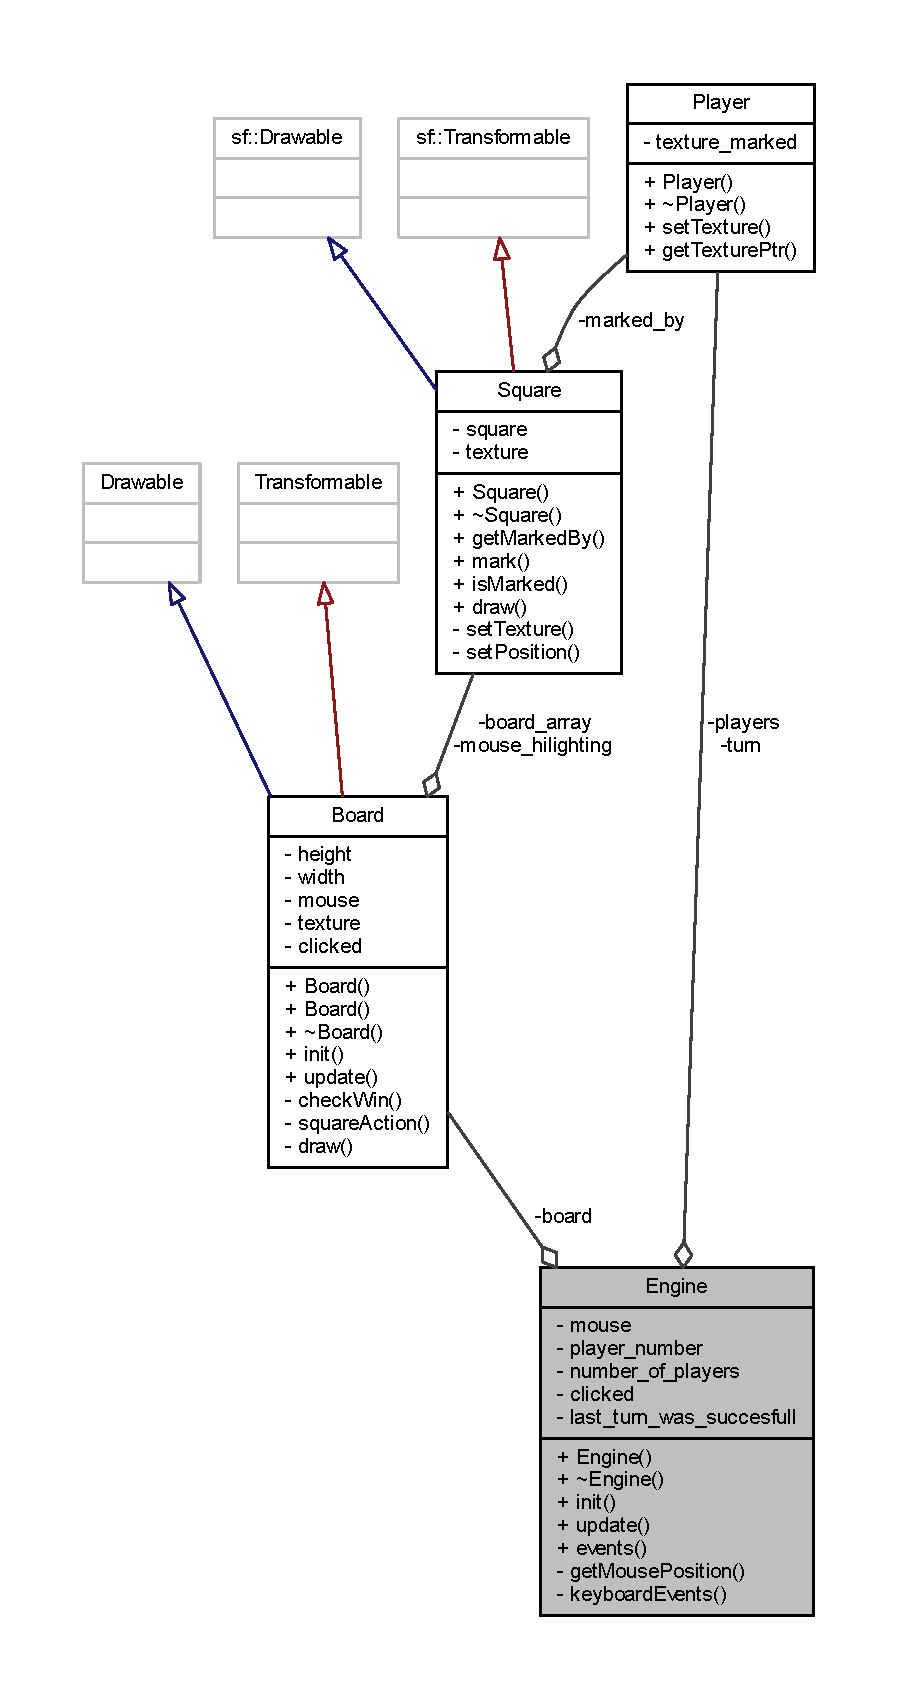
\includegraphics[height=550pt]{class_engine__coll__graph}
\end{center}
\end{figure}
\subsection*{Classes}
\begin{DoxyCompactItemize}
\item 
class \hyperlink{class_engine_1_1cpp}{cpp}
\end{DoxyCompactItemize}
\subsection*{Public Member Functions}
\begin{DoxyCompactItemize}
\item 
\hyperlink{class_engine_a8c98683b0a3aa28d8ab72a8bcd0d52f2}{Engine} ()
\begin{DoxyCompactList}\small\item\em sets vars to neutral state, pointers to N\+U\+L\+L \end{DoxyCompactList}\item 
virtual \hyperlink{class_engine_a8ef7030a089ecb30bbfcb9e43094717a}{$\sim$\+Engine} ()
\begin{DoxyCompactList}\small\item\em only debug msg \end{DoxyCompactList}\item 
void \hyperlink{class_engine_af4a62564ef402b7b5a8d880f05d5b120}{init} (sf\+::\+Render\+Window \&window)
\begin{DoxyCompactList}\small\item\em initialization of \hyperlink{class_engine}{Engine}, sets player textures \end{DoxyCompactList}\item 
void \hyperlink{class_engine_aaa07c6646868b4f752fbb91c3ec5380c}{update} (sf\+::\+Render\+Window \&window)
\item 
void \hyperlink{class_engine_a5c3c086eeec69ae6780eb0ffb5a9848e}{events} (sf\+::\+Render\+Window \&window, sf\+::\+Event \&event)
\begin{DoxyCompactList}\small\item\em updates physics of the game, draws board. \end{DoxyCompactList}\end{DoxyCompactItemize}
\subsection*{Private Member Functions}
\begin{DoxyCompactItemize}
\item 
void \hyperlink{class_engine_ac34480273d578527e8380758817e7bee}{get\+Mouse\+Position} (sf\+::\+Render\+Window \&window)
\begin{DoxyCompactList}\small\item\em gets global mouse position \end{DoxyCompactList}\item 
void \hyperlink{class_engine_af4b44a2dd17e35dfc5bb21917508627b}{keyboard\+Events} (sf\+::\+Render\+Window \&window, sf\+::\+Event \&event)
\begin{DoxyCompactList}\small\item\em reads keyboard events \end{DoxyCompactList}\end{DoxyCompactItemize}
\subsection*{Private Attributes}
\begin{DoxyCompactItemize}
\item 
\hyperlink{class_board}{Board} \hyperlink{class_engine_aab263540a0e814e6304a3ef6b751b097}{board}
\item 
sf\+::\+Vector2i \hyperlink{class_engine_a6da5d0a63da9f898192b2030b754065f}{mouse}
\begin{DoxyCompactList}\small\item\em contains dynamicly allocated array of squares \end{DoxyCompactList}\item 
\hyperlink{class_player}{Player} \hyperlink{class_engine_a2fd7bb89b1be2ea2a33e90e4d0699ffc}{players} \mbox{[}2\mbox{]}
\begin{DoxyCompactList}\small\item\em current mouse position \end{DoxyCompactList}\item 
\hyperlink{class_player}{Player} $\ast$ \hyperlink{class_engine_a747d5223870d541667213e307cc34d04}{turn}
\begin{DoxyCompactList}\small\item\em pointer to \hyperlink{class_player}{Player} whose turn it is \end{DoxyCompactList}\item 
int \hyperlink{class_engine_a663054b19f734fa167305abf546d8151}{player\+\_\+number}
\begin{DoxyCompactList}\small\item\em To fix . \end{DoxyCompactList}\item 
int \hyperlink{class_engine_a7c9d0480379dfdf9eafaf3344d076e4d}{number\+\_\+of\+\_\+players}
\begin{DoxyCompactList}\small\item\em number of players \end{DoxyCompactList}\item 
bool \hyperlink{class_engine_a9c9336f739cd336a1346a17504857a45}{clicked}
\begin{DoxyCompactList}\small\item\em var if lmouse button was clicked true else false \end{DoxyCompactList}\item 
bool \hyperlink{class_engine_a7dbc1e409179b77add60013155b684a0}{last\+\_\+turn\+\_\+was\+\_\+succesfull}
\begin{DoxyCompactList}\small\item\em true if last turn was successful (no illegal action like marking already marked square) \end{DoxyCompactList}\end{DoxyCompactItemize}


\subsection{Detailed Description}
\hyperlink{class_engine}{Engine} class. Class which manage main loop of game, reads keyboard events, update physics. This class will menage menu and settings. 

\subsection{Constructor \& Destructor Documentation}
\hypertarget{class_engine_a8c98683b0a3aa28d8ab72a8bcd0d52f2}{}\index{Engine@{Engine}!Engine@{Engine}}
\index{Engine@{Engine}!Engine@{Engine}}
\subsubsection[{Engine}]{\setlength{\rightskip}{0pt plus 5cm}Engine\+::\+Engine (
\begin{DoxyParamCaption}
{}
\end{DoxyParamCaption}
)}\label{class_engine_a8c98683b0a3aa28d8ab72a8bcd0d52f2}


sets vars to neutral state, pointers to N\+U\+L\+L 

\hypertarget{class_engine_a8ef7030a089ecb30bbfcb9e43094717a}{}\index{Engine@{Engine}!````~Engine@{$\sim$\+Engine}}
\index{````~Engine@{$\sim$\+Engine}!Engine@{Engine}}
\subsubsection[{$\sim$\+Engine}]{\setlength{\rightskip}{0pt plus 5cm}Engine\+::$\sim$\+Engine (
\begin{DoxyParamCaption}
{}
\end{DoxyParamCaption}
)\hspace{0.3cm}{\ttfamily [virtual]}}\label{class_engine_a8ef7030a089ecb30bbfcb9e43094717a}


only debug msg 



\subsection{Member Function Documentation}
\hypertarget{class_engine_a5c3c086eeec69ae6780eb0ffb5a9848e}{}\index{Engine@{Engine}!events@{events}}
\index{events@{events}!Engine@{Engine}}
\subsubsection[{events}]{\setlength{\rightskip}{0pt plus 5cm}void Engine\+::events (
\begin{DoxyParamCaption}
\item[{sf\+::\+Render\+Window \&}]{window, }
\item[{sf\+::\+Event \&}]{event}
\end{DoxyParamCaption}
)}\label{class_engine_a5c3c086eeec69ae6780eb0ffb5a9848e}


updates physics of the game, draws board. 

reads events all 

Here is the call graph for this function\+:\nopagebreak
\begin{figure}[H]
\begin{center}
\leavevmode
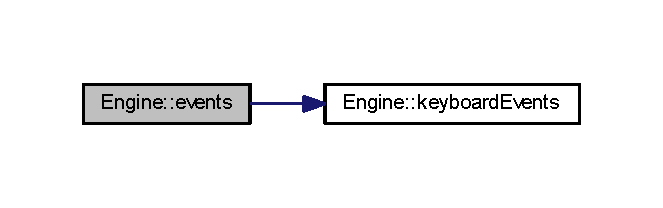
\includegraphics[width=318pt]{class_engine_a5c3c086eeec69ae6780eb0ffb5a9848e_cgraph}
\end{center}
\end{figure}




Here is the caller graph for this function\+:\nopagebreak
\begin{figure}[H]
\begin{center}
\leavevmode
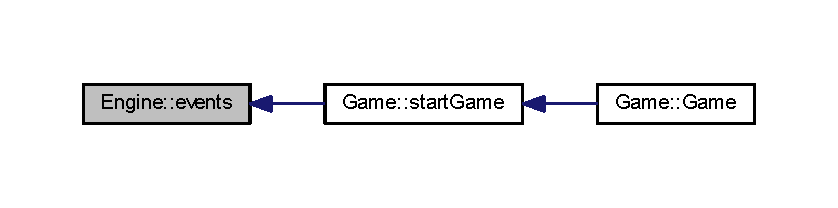
\includegraphics[width=350pt]{class_engine_a5c3c086eeec69ae6780eb0ffb5a9848e_icgraph}
\end{center}
\end{figure}


\hypertarget{class_engine_ac34480273d578527e8380758817e7bee}{}\index{Engine@{Engine}!get\+Mouse\+Position@{get\+Mouse\+Position}}
\index{get\+Mouse\+Position@{get\+Mouse\+Position}!Engine@{Engine}}
\subsubsection[{get\+Mouse\+Position}]{\setlength{\rightskip}{0pt plus 5cm}void Engine\+::get\+Mouse\+Position (
\begin{DoxyParamCaption}
\item[{sf\+::\+Render\+Window \&}]{window}
\end{DoxyParamCaption}
)\hspace{0.3cm}{\ttfamily [private]}}\label{class_engine_ac34480273d578527e8380758817e7bee}


gets global mouse position 



Here is the caller graph for this function\+:\nopagebreak
\begin{figure}[H]
\begin{center}
\leavevmode
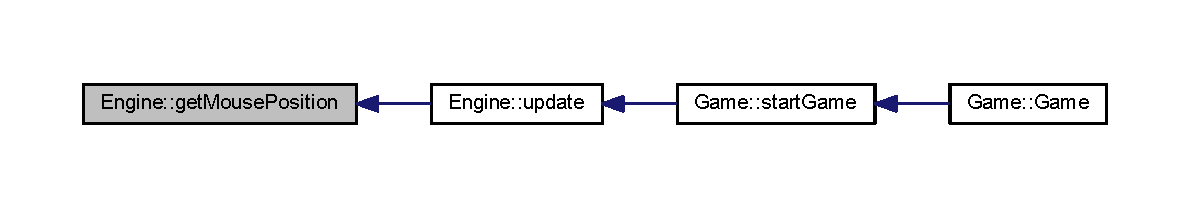
\includegraphics[width=350pt]{class_engine_ac34480273d578527e8380758817e7bee_icgraph}
\end{center}
\end{figure}


\hypertarget{class_engine_af4a62564ef402b7b5a8d880f05d5b120}{}\index{Engine@{Engine}!init@{init}}
\index{init@{init}!Engine@{Engine}}
\subsubsection[{init}]{\setlength{\rightskip}{0pt plus 5cm}void Engine\+::init (
\begin{DoxyParamCaption}
\item[{sf\+::\+Render\+Window \&}]{window}
\end{DoxyParamCaption}
)}\label{class_engine_af4a62564ef402b7b5a8d880f05d5b120}


initialization of \hyperlink{class_engine}{Engine}, sets player textures 



Here is the call graph for this function\+:\nopagebreak
\begin{figure}[H]
\begin{center}
\leavevmode
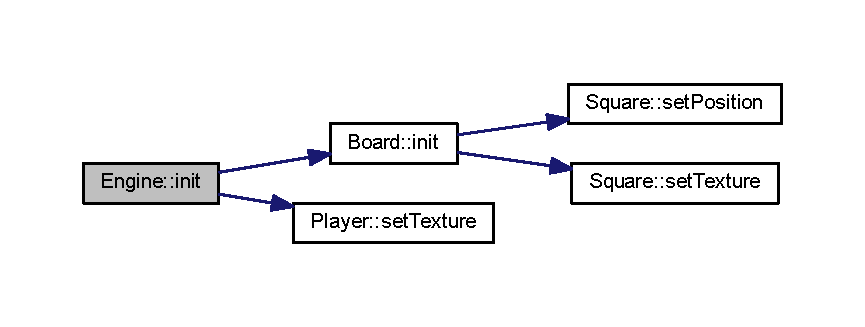
\includegraphics[width=350pt]{class_engine_af4a62564ef402b7b5a8d880f05d5b120_cgraph}
\end{center}
\end{figure}




Here is the caller graph for this function\+:\nopagebreak
\begin{figure}[H]
\begin{center}
\leavevmode
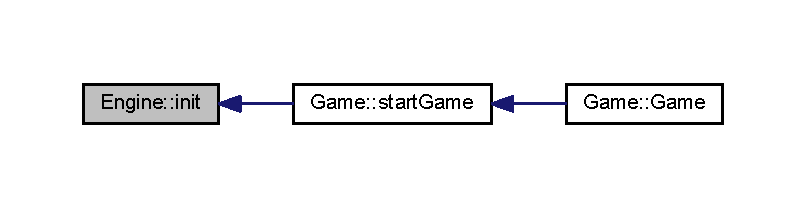
\includegraphics[width=350pt]{class_engine_af4a62564ef402b7b5a8d880f05d5b120_icgraph}
\end{center}
\end{figure}


\hypertarget{class_engine_af4b44a2dd17e35dfc5bb21917508627b}{}\index{Engine@{Engine}!keyboard\+Events@{keyboard\+Events}}
\index{keyboard\+Events@{keyboard\+Events}!Engine@{Engine}}
\subsubsection[{keyboard\+Events}]{\setlength{\rightskip}{0pt plus 5cm}void Engine\+::keyboard\+Events (
\begin{DoxyParamCaption}
\item[{sf\+::\+Render\+Window \&}]{window, }
\item[{sf\+::\+Event \&}]{event}
\end{DoxyParamCaption}
)\hspace{0.3cm}{\ttfamily [private]}}\label{class_engine_af4b44a2dd17e35dfc5bb21917508627b}


reads keyboard events 



Here is the caller graph for this function\+:\nopagebreak
\begin{figure}[H]
\begin{center}
\leavevmode
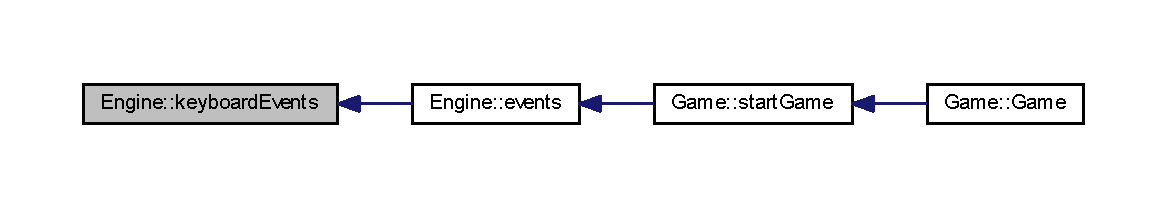
\includegraphics[width=350pt]{class_engine_af4b44a2dd17e35dfc5bb21917508627b_icgraph}
\end{center}
\end{figure}


\hypertarget{class_engine_aaa07c6646868b4f752fbb91c3ec5380c}{}\index{Engine@{Engine}!update@{update}}
\index{update@{update}!Engine@{Engine}}
\subsubsection[{update}]{\setlength{\rightskip}{0pt plus 5cm}void Engine\+::update (
\begin{DoxyParamCaption}
\item[{sf\+::\+Render\+Window \&}]{window}
\end{DoxyParamCaption}
)}\label{class_engine_aaa07c6646868b4f752fbb91c3ec5380c}
unfortunatlly changes when there were player turn failed 

Here is the call graph for this function\+:
\nopagebreak
\begin{figure}[H]
\begin{center}
\leavevmode
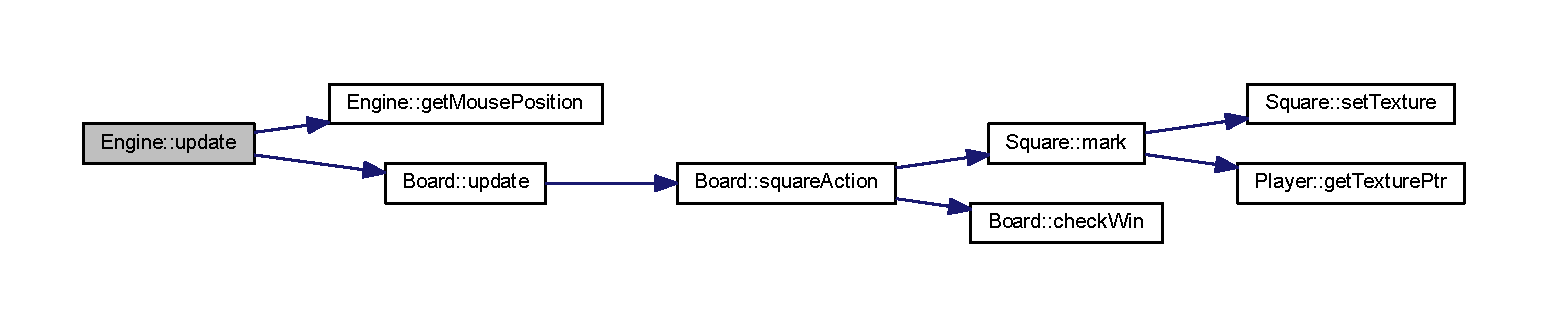
\includegraphics[width=350pt]{class_engine_aaa07c6646868b4f752fbb91c3ec5380c_cgraph}
\end{center}
\end{figure}




Here is the caller graph for this function\+:\nopagebreak
\begin{figure}[H]
\begin{center}
\leavevmode
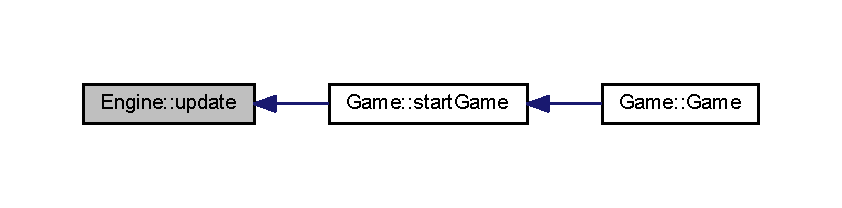
\includegraphics[width=350pt]{class_engine_aaa07c6646868b4f752fbb91c3ec5380c_icgraph}
\end{center}
\end{figure}




\subsection{Member Data Documentation}
\hypertarget{class_engine_aab263540a0e814e6304a3ef6b751b097}{}\index{Engine@{Engine}!board@{board}}
\index{board@{board}!Engine@{Engine}}
\subsubsection[{board}]{\setlength{\rightskip}{0pt plus 5cm}{\bf Board} Engine\+::board\hspace{0.3cm}{\ttfamily [private]}}\label{class_engine_aab263540a0e814e6304a3ef6b751b097}
\hypertarget{class_engine_a9c9336f739cd336a1346a17504857a45}{}\index{Engine@{Engine}!clicked@{clicked}}
\index{clicked@{clicked}!Engine@{Engine}}
\subsubsection[{clicked}]{\setlength{\rightskip}{0pt plus 5cm}bool Engine\+::clicked\hspace{0.3cm}{\ttfamily [private]}}\label{class_engine_a9c9336f739cd336a1346a17504857a45}


var if lmouse button was clicked true else false 

\hypertarget{class_engine_a7dbc1e409179b77add60013155b684a0}{}\index{Engine@{Engine}!last\+\_\+turn\+\_\+was\+\_\+succesfull@{last\+\_\+turn\+\_\+was\+\_\+succesfull}}
\index{last\+\_\+turn\+\_\+was\+\_\+succesfull@{last\+\_\+turn\+\_\+was\+\_\+succesfull}!Engine@{Engine}}
\subsubsection[{last\+\_\+turn\+\_\+was\+\_\+succesfull}]{\setlength{\rightskip}{0pt plus 5cm}bool Engine\+::last\+\_\+turn\+\_\+was\+\_\+succesfull\hspace{0.3cm}{\ttfamily [private]}}\label{class_engine_a7dbc1e409179b77add60013155b684a0}


true if last turn was successful (no illegal action like marking already marked square) 

\hypertarget{class_engine_a6da5d0a63da9f898192b2030b754065f}{}\index{Engine@{Engine}!mouse@{mouse}}
\index{mouse@{mouse}!Engine@{Engine}}
\subsubsection[{mouse}]{\setlength{\rightskip}{0pt plus 5cm}sf\+::\+Vector2i Engine\+::mouse\hspace{0.3cm}{\ttfamily [private]}}\label{class_engine_a6da5d0a63da9f898192b2030b754065f}


contains dynamicly allocated array of squares 

\hypertarget{class_engine_a7c9d0480379dfdf9eafaf3344d076e4d}{}\index{Engine@{Engine}!number\+\_\+of\+\_\+players@{number\+\_\+of\+\_\+players}}
\index{number\+\_\+of\+\_\+players@{number\+\_\+of\+\_\+players}!Engine@{Engine}}
\subsubsection[{number\+\_\+of\+\_\+players}]{\setlength{\rightskip}{0pt plus 5cm}int Engine\+::number\+\_\+of\+\_\+players\hspace{0.3cm}{\ttfamily [private]}}\label{class_engine_a7c9d0480379dfdf9eafaf3344d076e4d}


number of players 

\hypertarget{class_engine_a663054b19f734fa167305abf546d8151}{}\index{Engine@{Engine}!player\+\_\+number@{player\+\_\+number}}
\index{player\+\_\+number@{player\+\_\+number}!Engine@{Engine}}
\subsubsection[{player\+\_\+number}]{\setlength{\rightskip}{0pt plus 5cm}int Engine\+::player\+\_\+number\hspace{0.3cm}{\ttfamily [private]}}\label{class_engine_a663054b19f734fa167305abf546d8151}


To fix . 

\hypertarget{class_engine_a2fd7bb89b1be2ea2a33e90e4d0699ffc}{}\index{Engine@{Engine}!players@{players}}
\index{players@{players}!Engine@{Engine}}
\subsubsection[{players}]{\setlength{\rightskip}{0pt plus 5cm}{\bf Player} Engine\+::players\mbox{[}2\mbox{]}\hspace{0.3cm}{\ttfamily [private]}}\label{class_engine_a2fd7bb89b1be2ea2a33e90e4d0699ffc}


current mouse position 

just for tests array of players \hypertarget{class_engine_a747d5223870d541667213e307cc34d04}{}\index{Engine@{Engine}!turn@{turn}}
\index{turn@{turn}!Engine@{Engine}}
\subsubsection[{turn}]{\setlength{\rightskip}{0pt plus 5cm}{\bf Player}$\ast$ Engine\+::turn\hspace{0.3cm}{\ttfamily [private]}}\label{class_engine_a747d5223870d541667213e307cc34d04}


pointer to \hyperlink{class_player}{Player} whose turn it is 



The documentation for this class was generated from the following files\+:\begin{DoxyCompactItemize}
\item 
\hyperlink{_engine_8h}{Engine.\+h}\item 
\hyperlink{_engine_8cpp}{Engine.\+cpp}\end{DoxyCompactItemize}

\hypertarget{class_game}{}\section{Game Class Reference}
\label{class_game}\index{Game@{Game}}


\hyperlink{class_game}{Game} main class. Class which is used run engine. This class will menage menu and settings.  




{\ttfamily \#include $<$Game.\+h$>$}



Collaboration diagram for Game\+:
\nopagebreak
\begin{figure}[H]
\begin{center}
\leavevmode
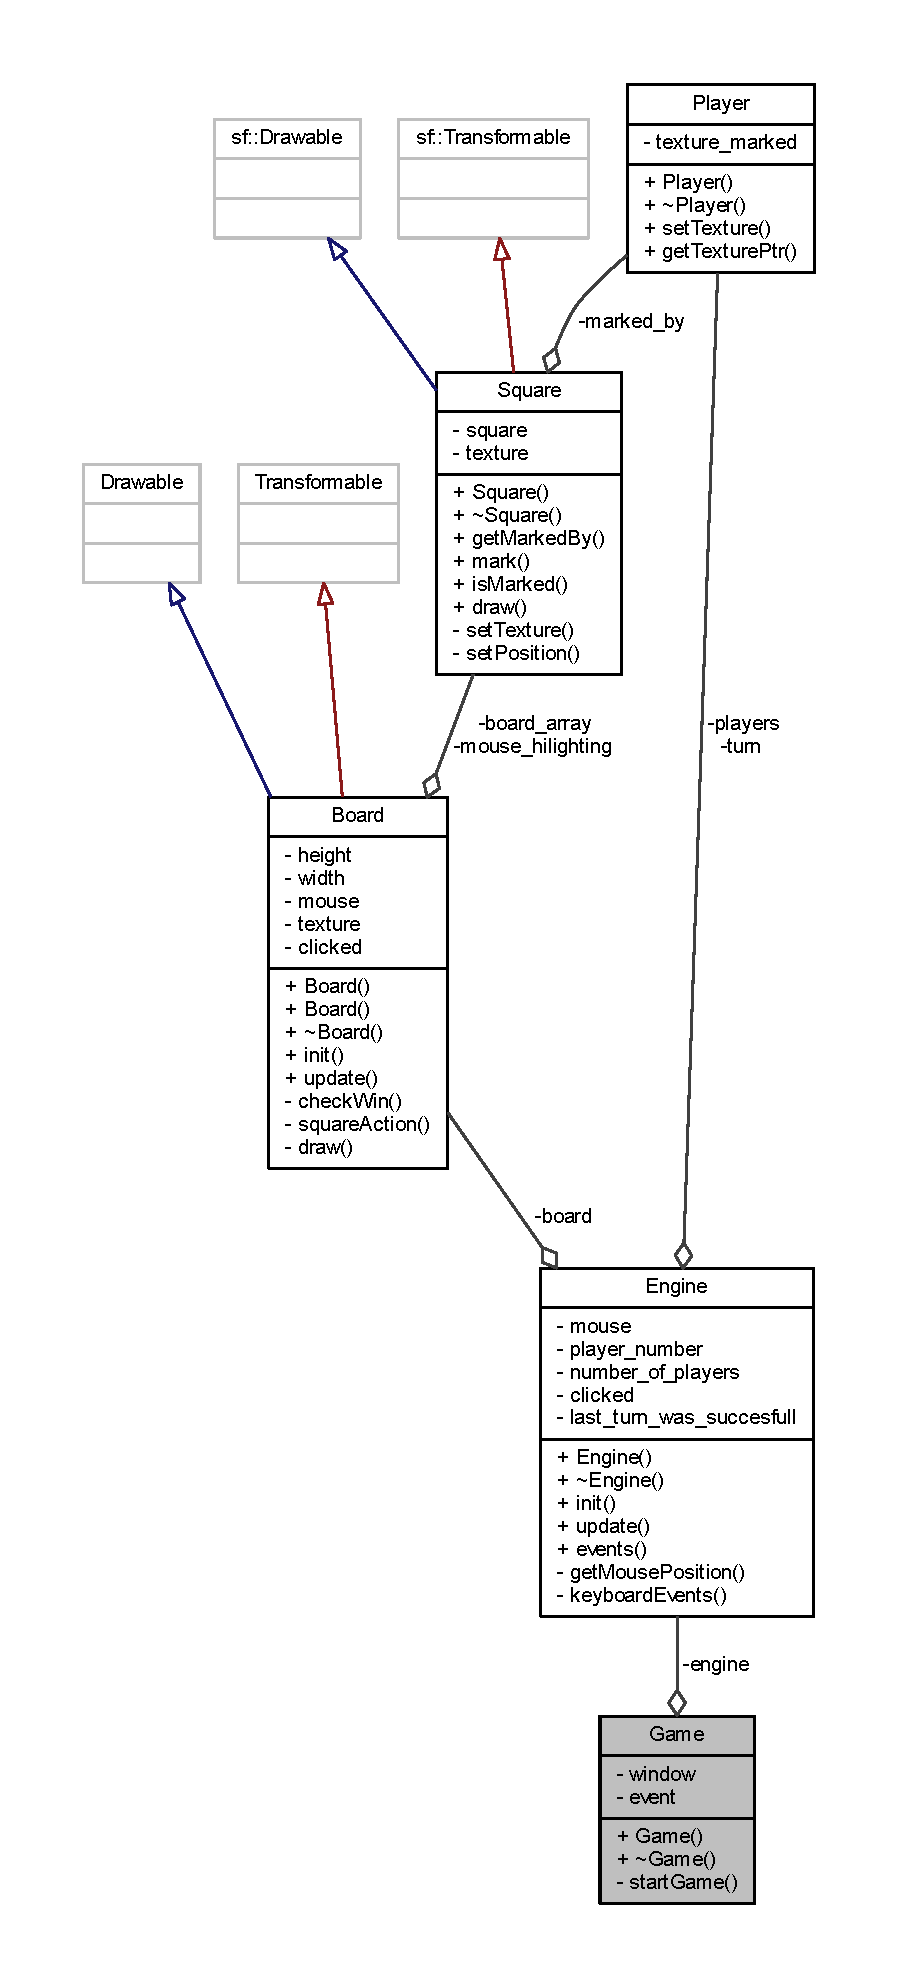
\includegraphics[height=550pt]{class_game__coll__graph}
\end{center}
\end{figure}
\subsection*{Public Member Functions}
\begin{DoxyCompactItemize}
\item 
\hyperlink{class_game_af4259d9962bf0998d01c6e594eca2f58}{Game} (sf\+::\+Render\+Window \&\hyperlink{class_game_ad0fb4d8653dcf289fd6573cf5ba0f3d1}{window})
\begin{DoxyCompactList}\small\item\em Initialization of Render\+Window\& window -\/ main window of the game. \end{DoxyCompactList}\item 
virtual \hyperlink{class_game_ae3d112ca6e0e55150d2fdbc704474530}{$\sim$\+Game} ()
\begin{DoxyCompactList}\small\item\em Runs Start\+Game() function. \end{DoxyCompactList}\end{DoxyCompactItemize}
\subsection*{Private Member Functions}
\begin{DoxyCompactItemize}
\item 
void \hyperlink{class_game_ae8638ccdb0ef3bf39a6affa30aa1258f}{start\+Game} ()
\begin{DoxyCompactList}\small\item\em Runs engine starts multi player seats switch game. \end{DoxyCompactList}\end{DoxyCompactItemize}
\subsection*{Private Attributes}
\begin{DoxyCompactItemize}
\item 
\hyperlink{class_engine}{Engine} \hyperlink{class_game_ad407022fcdd5ece2ccb8ae9ab6558a73}{engine}
\begin{DoxyCompactList}\small\item\em Main engine of the game. \end{DoxyCompactList}\item 
sf\+::\+Render\+Window \& \hyperlink{class_game_ad0fb4d8653dcf289fd6573cf5ba0f3d1}{window}
\begin{DoxyCompactList}\small\item\em Main game window. \end{DoxyCompactList}\item 
sf\+::\+Event \hyperlink{class_game_a399e6ac5b37307b16dc9f769e0b538c9}{event}
\begin{DoxyCompactList}\small\item\em Event object probably unused. \end{DoxyCompactList}\end{DoxyCompactItemize}


\subsection{Detailed Description}
\hyperlink{class_game}{Game} main class. Class which is used run engine. This class will menage menu and settings. 

\subsection{Constructor \& Destructor Documentation}
\hypertarget{class_game_af4259d9962bf0998d01c6e594eca2f58}{}\index{Game@{Game}!Game@{Game}}
\index{Game@{Game}!Game@{Game}}
\subsubsection[{Game}]{\setlength{\rightskip}{0pt plus 5cm}Game\+::\+Game (
\begin{DoxyParamCaption}
\item[{sf\+::\+Render\+Window \&}]{window}
\end{DoxyParamCaption}
)}\label{class_game_af4259d9962bf0998d01c6e594eca2f58}


Initialization of Render\+Window\& window -\/ main window of the game. 



Here is the call graph for this function\+:
\nopagebreak
\begin{figure}[H]
\begin{center}
\leavevmode
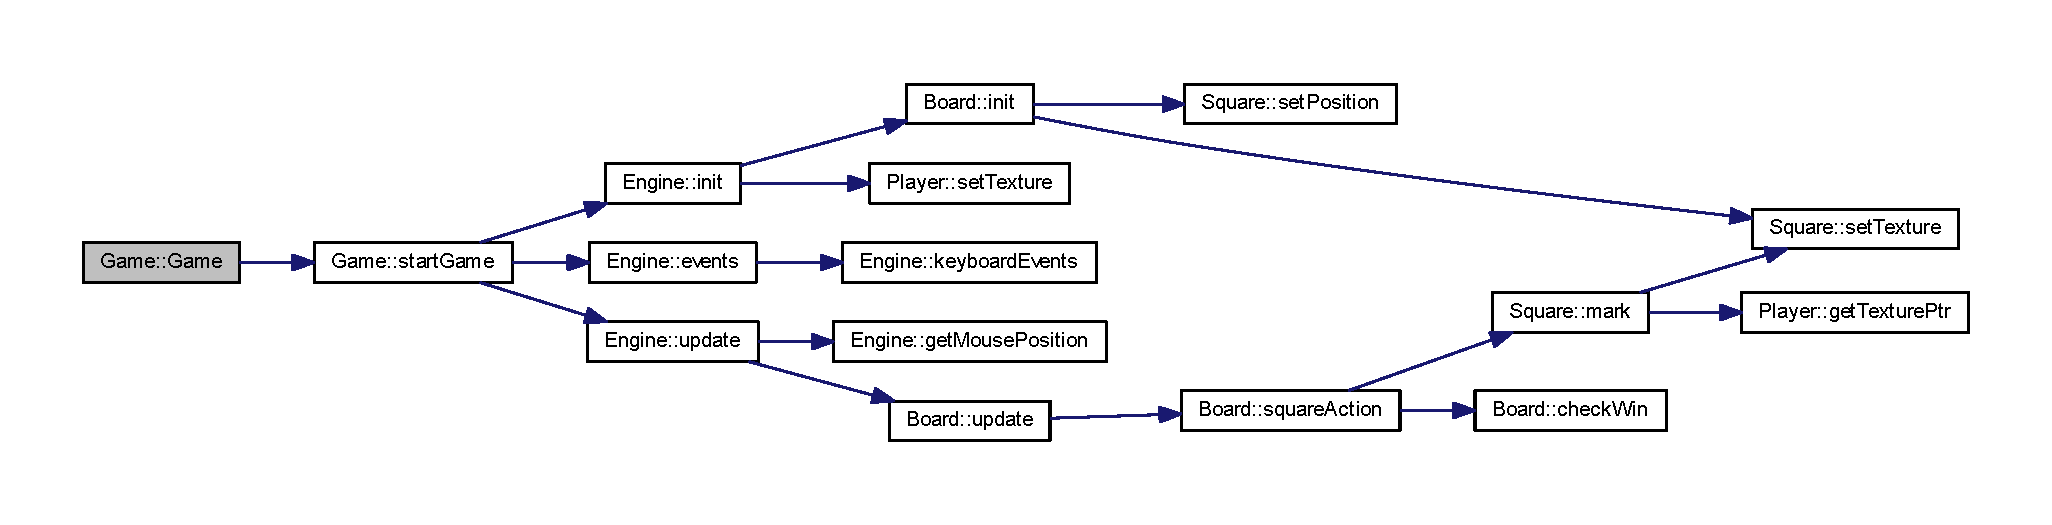
\includegraphics[width=350pt]{class_game_af4259d9962bf0998d01c6e594eca2f58_cgraph}
\end{center}
\end{figure}


\hypertarget{class_game_ae3d112ca6e0e55150d2fdbc704474530}{}\index{Game@{Game}!````~Game@{$\sim$\+Game}}
\index{````~Game@{$\sim$\+Game}!Game@{Game}}
\subsubsection[{$\sim$\+Game}]{\setlength{\rightskip}{0pt plus 5cm}Game\+::$\sim$\+Game (
\begin{DoxyParamCaption}
{}
\end{DoxyParamCaption}
)\hspace{0.3cm}{\ttfamily [virtual]}}\label{class_game_ae3d112ca6e0e55150d2fdbc704474530}


Runs Start\+Game() function. 



\subsection{Member Function Documentation}
\hypertarget{class_game_ae8638ccdb0ef3bf39a6affa30aa1258f}{}\index{Game@{Game}!start\+Game@{start\+Game}}
\index{start\+Game@{start\+Game}!Game@{Game}}
\subsubsection[{start\+Game}]{\setlength{\rightskip}{0pt plus 5cm}void Game\+::start\+Game (
\begin{DoxyParamCaption}
{}
\end{DoxyParamCaption}
)\hspace{0.3cm}{\ttfamily [private]}}\label{class_game_ae8638ccdb0ef3bf39a6affa30aa1258f}


Runs engine starts multi player seats switch game. 



Here is the call graph for this function\+:
\nopagebreak
\begin{figure}[H]
\begin{center}
\leavevmode
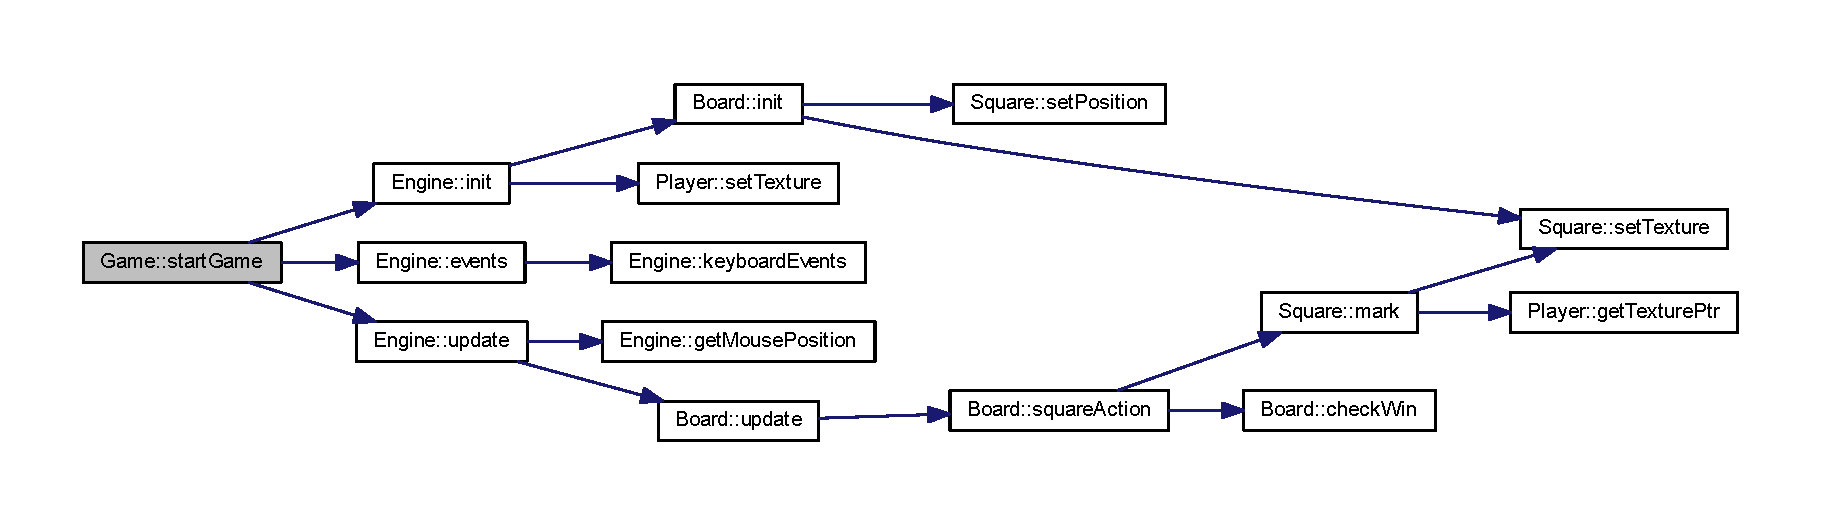
\includegraphics[width=350pt]{class_game_ae8638ccdb0ef3bf39a6affa30aa1258f_cgraph}
\end{center}
\end{figure}




Here is the caller graph for this function\+:\nopagebreak
\begin{figure}[H]
\begin{center}
\leavevmode
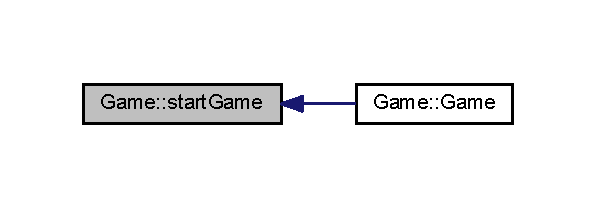
\includegraphics[width=286pt]{class_game_ae8638ccdb0ef3bf39a6affa30aa1258f_icgraph}
\end{center}
\end{figure}




\subsection{Member Data Documentation}
\hypertarget{class_game_ad407022fcdd5ece2ccb8ae9ab6558a73}{}\index{Game@{Game}!engine@{engine}}
\index{engine@{engine}!Game@{Game}}
\subsubsection[{engine}]{\setlength{\rightskip}{0pt plus 5cm}{\bf Engine} Game\+::engine\hspace{0.3cm}{\ttfamily [private]}}\label{class_game_ad407022fcdd5ece2ccb8ae9ab6558a73}


Main engine of the game. 

\hypertarget{class_game_a399e6ac5b37307b16dc9f769e0b538c9}{}\index{Game@{Game}!event@{event}}
\index{event@{event}!Game@{Game}}
\subsubsection[{event}]{\setlength{\rightskip}{0pt plus 5cm}sf\+::\+Event Game\+::event\hspace{0.3cm}{\ttfamily [private]}}\label{class_game_a399e6ac5b37307b16dc9f769e0b538c9}


Event object probably unused. 

\hypertarget{class_game_ad0fb4d8653dcf289fd6573cf5ba0f3d1}{}\index{Game@{Game}!window@{window}}
\index{window@{window}!Game@{Game}}
\subsubsection[{window}]{\setlength{\rightskip}{0pt plus 5cm}sf\+::\+Render\+Window\& Game\+::window\hspace{0.3cm}{\ttfamily [private]}}\label{class_game_ad0fb4d8653dcf289fd6573cf5ba0f3d1}


Main game window. 



The documentation for this class was generated from the following files\+:\begin{DoxyCompactItemize}
\item 
\hyperlink{_game_8h}{Game.\+h}\item 
\hyperlink{_game_8cpp}{Game.\+cpp}\end{DoxyCompactItemize}

\hypertarget{class_player}{}\section{Player Class Reference}
\label{class_player}\index{Player@{Player}}


\hyperlink{class_player}{Player} class -\/ pointers to player have a lot of usage in program. All Squares have pointer to player which were marked by pointers to players are also used by \hyperlink{class_engine}{Engine} class to set whose turn is now.  




{\ttfamily \#include $<$Player.\+h$>$}



Collaboration diagram for Player\+:
\nopagebreak
\begin{figure}[H]
\begin{center}
\leavevmode
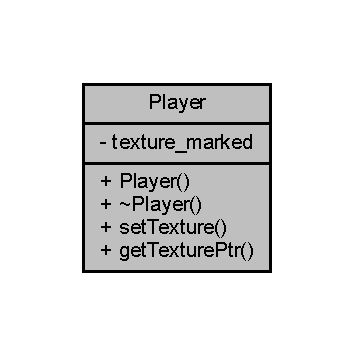
\includegraphics[width=170pt]{class_player__coll__graph}
\end{center}
\end{figure}
\subsection*{Public Member Functions}
\begin{DoxyCompactItemize}
\item 
\hyperlink{class_player_affe0cc3cb714f6deb4e62f0c0d3f1fd8}{Player} ()
\begin{DoxyCompactList}\small\item\em empty constructor \end{DoxyCompactList}\item 
virtual \hyperlink{class_player_a749d2c00e1fe0f5c2746f7505a58c062}{$\sim$\+Player} ()
\begin{DoxyCompactList}\small\item\em empty destructor only msg \end{DoxyCompactList}\item 
void \hyperlink{class_player_ac2412646697fb7738a5d0c3aeb16ba94}{set\+Texture} (char $\ast$file\+Dir)
\begin{DoxyCompactList}\small\item\em function setting player texture (initialization staff) \end{DoxyCompactList}\item 
sf\+::\+Texture $\ast$ \hyperlink{class_player_a72e351147bd2bb48bdea9ba74dcc7f81}{get\+Texture\+Ptr} ()
\begin{DoxyCompactList}\small\item\em returns pointer to current player texture (texture\+\_\+marked) \end{DoxyCompactList}\end{DoxyCompactItemize}
\subsection*{Private Attributes}
\begin{DoxyCompactItemize}
\item 
sf\+::\+Texture \hyperlink{class_player_a9e50410dd4405082cc4374126e813a95}{texture\+\_\+marked}
\begin{DoxyCompactList}\small\item\em texture to draw when a player marked square. \end{DoxyCompactList}\end{DoxyCompactItemize}


\subsection{Detailed Description}
\hyperlink{class_player}{Player} class -\/ pointers to player have a lot of usage in program. All Squares have pointer to player which were marked by pointers to players are also used by \hyperlink{class_engine}{Engine} class to set whose turn is now. 

\subsection{Constructor \& Destructor Documentation}
\hypertarget{class_player_affe0cc3cb714f6deb4e62f0c0d3f1fd8}{}\index{Player@{Player}!Player@{Player}}
\index{Player@{Player}!Player@{Player}}
\subsubsection[{Player}]{\setlength{\rightskip}{0pt plus 5cm}Player\+::\+Player (
\begin{DoxyParamCaption}
{}
\end{DoxyParamCaption}
)}\label{class_player_affe0cc3cb714f6deb4e62f0c0d3f1fd8}


empty constructor 

\hypertarget{class_player_a749d2c00e1fe0f5c2746f7505a58c062}{}\index{Player@{Player}!````~Player@{$\sim$\+Player}}
\index{````~Player@{$\sim$\+Player}!Player@{Player}}
\subsubsection[{$\sim$\+Player}]{\setlength{\rightskip}{0pt plus 5cm}Player\+::$\sim$\+Player (
\begin{DoxyParamCaption}
{}
\end{DoxyParamCaption}
)\hspace{0.3cm}{\ttfamily [virtual]}}\label{class_player_a749d2c00e1fe0f5c2746f7505a58c062}


empty destructor only msg 



\subsection{Member Function Documentation}
\hypertarget{class_player_a72e351147bd2bb48bdea9ba74dcc7f81}{}\index{Player@{Player}!get\+Texture\+Ptr@{get\+Texture\+Ptr}}
\index{get\+Texture\+Ptr@{get\+Texture\+Ptr}!Player@{Player}}
\subsubsection[{get\+Texture\+Ptr}]{\setlength{\rightskip}{0pt plus 5cm}sf\+::\+Texture $\ast$ Player\+::get\+Texture\+Ptr (
\begin{DoxyParamCaption}
{}
\end{DoxyParamCaption}
)}\label{class_player_a72e351147bd2bb48bdea9ba74dcc7f81}


returns pointer to current player texture (texture\+\_\+marked) 



Here is the caller graph for this function\+:
\nopagebreak
\begin{figure}[H]
\begin{center}
\leavevmode
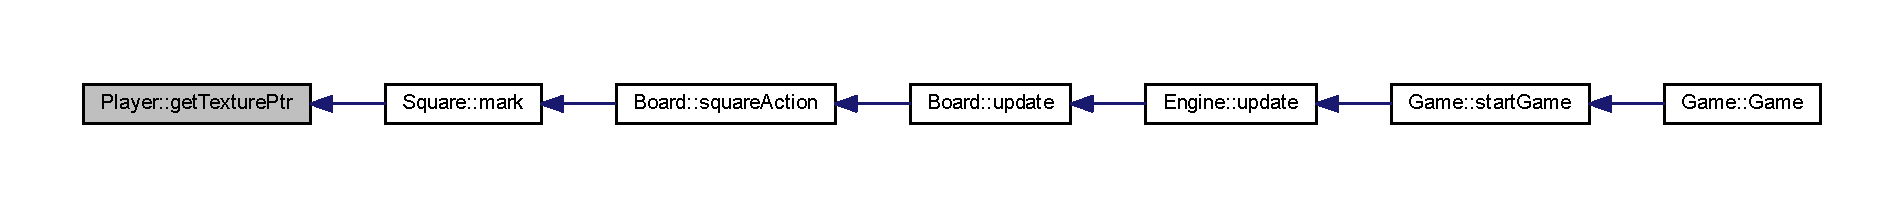
\includegraphics[width=350pt]{class_player_a72e351147bd2bb48bdea9ba74dcc7f81_icgraph}
\end{center}
\end{figure}


\hypertarget{class_player_ac2412646697fb7738a5d0c3aeb16ba94}{}\index{Player@{Player}!set\+Texture@{set\+Texture}}
\index{set\+Texture@{set\+Texture}!Player@{Player}}
\subsubsection[{set\+Texture}]{\setlength{\rightskip}{0pt plus 5cm}void Player\+::set\+Texture (
\begin{DoxyParamCaption}
\item[{char $\ast$}]{file\+Dir}
\end{DoxyParamCaption}
)}\label{class_player_ac2412646697fb7738a5d0c3aeb16ba94}


function setting player texture (initialization staff) 



Here is the caller graph for this function\+:\nopagebreak
\begin{figure}[H]
\begin{center}
\leavevmode
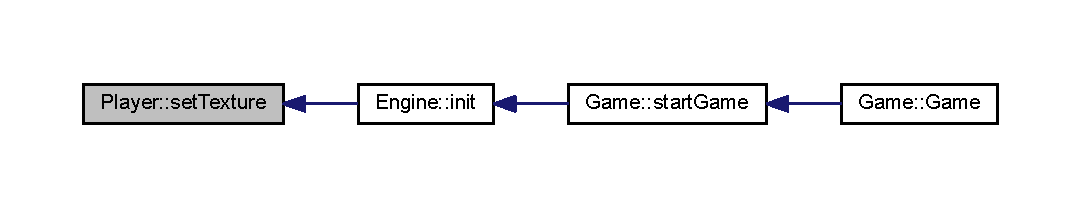
\includegraphics[width=350pt]{class_player_ac2412646697fb7738a5d0c3aeb16ba94_icgraph}
\end{center}
\end{figure}




\subsection{Member Data Documentation}
\hypertarget{class_player_a9e50410dd4405082cc4374126e813a95}{}\index{Player@{Player}!texture\+\_\+marked@{texture\+\_\+marked}}
\index{texture\+\_\+marked@{texture\+\_\+marked}!Player@{Player}}
\subsubsection[{texture\+\_\+marked}]{\setlength{\rightskip}{0pt plus 5cm}sf\+::\+Texture Player\+::texture\+\_\+marked\hspace{0.3cm}{\ttfamily [private]}}\label{class_player_a9e50410dd4405082cc4374126e813a95}


texture to draw when a player marked square. 



The documentation for this class was generated from the following files\+:\begin{DoxyCompactItemize}
\item 
\hyperlink{_player_8h}{Player.\+h}\item 
\hyperlink{_player_8cpp}{Player.\+cpp}\end{DoxyCompactItemize}

\hypertarget{class_square}{}\section{Square Class Reference}
\label{class_square}\index{Square@{Square}}


\hyperlink{class_square}{Square} class. Class which is used to build board this class may be remade to inheritance from sf\+::\+Rectangle\+Shape.  




{\ttfamily \#include $<$Square.\+h$>$}



Inheritance diagram for Square\+:
\nopagebreak
\begin{figure}[H]
\begin{center}
\leavevmode
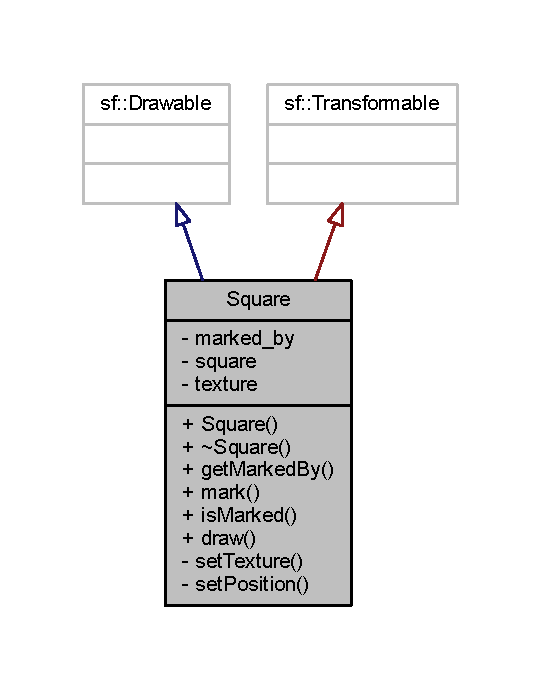
\includegraphics[width=260pt]{class_square__inherit__graph}
\end{center}
\end{figure}


Collaboration diagram for Square\+:
\nopagebreak
\begin{figure}[H]
\begin{center}
\leavevmode
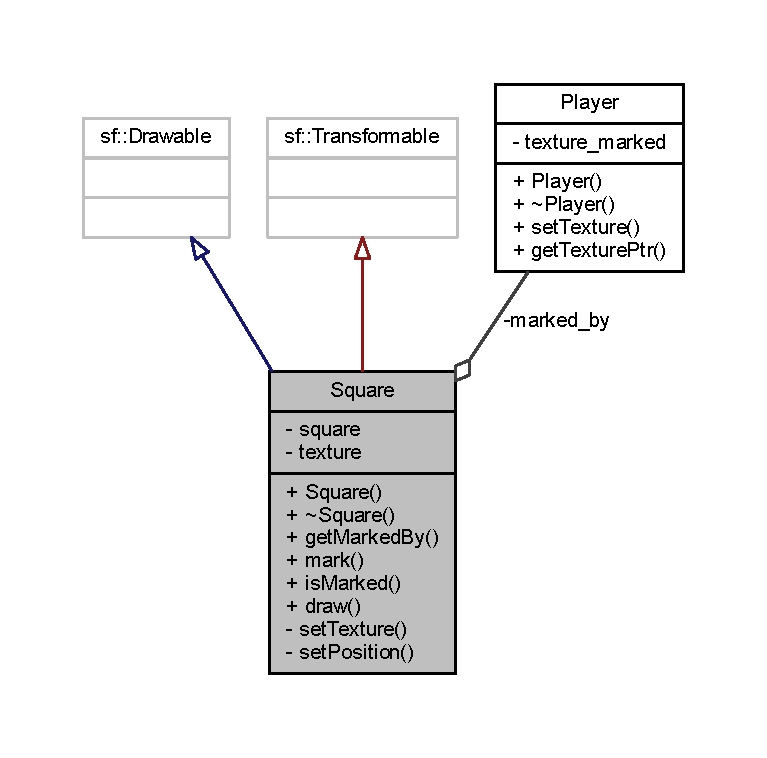
\includegraphics[width=350pt]{class_square__coll__graph}
\end{center}
\end{figure}
\subsection*{Public Member Functions}
\begin{DoxyCompactItemize}
\item 
\hyperlink{class_square_a3dc7ff9aefc2725172b5d3153973d243}{Square} ()
\begin{DoxyCompactList}\small\item\em sets pointers to N\+U\+L\+L \end{DoxyCompactList}\item 
virtual \hyperlink{class_square_a90af7ce1060cff7b717ceddb333846b8}{$\sim$\+Square} ()
\begin{DoxyCompactList}\small\item\em only D\+E\+B\+U\+G M\+S\+G \end{DoxyCompactList}\item 
\hyperlink{class_player}{Player} $\ast$ \hyperlink{class_square_ab67268190c292712504e4a6039781423}{get\+Marked\+By} () const 
\begin{DoxyCompactList}\small\item\em function returning pointer to \hyperlink{class_player}{Player} whose marked this \hyperlink{class_square}{Square}(var -\/ marked\+\_\+by) \end{DoxyCompactList}\item 
void \hyperlink{class_square_ab425c2f7271014c9d01eff4b0e053b31}{mark} (\hyperlink{class_player}{Player} $\ast$player\+\_\+ptr)
\begin{DoxyCompactList}\small\item\em this is function used by \hyperlink{class_board}{Board} to set \hyperlink{class_square}{Square} marked \end{DoxyCompactList}\item 
bool \hyperlink{class_square_a0b6ff04d5e7f6349889e989c6c187672}{is\+Marked} () const 
\begin{DoxyCompactList}\small\item\em returns true if square is marked(to rework) \end{DoxyCompactList}\item 
virtual void \hyperlink{class_square_a343e5c679cacddf7250f363875518bf9}{draw} (sf\+::\+Render\+Target \&target, sf\+::\+Render\+States states) const 
\begin{DoxyCompactList}\small\item\em draws sf\+::\+Rectangle\+Shape square \end{DoxyCompactList}\end{DoxyCompactItemize}
\subsection*{Private Member Functions}
\begin{DoxyCompactItemize}
\item 
void \hyperlink{class_square_ad62196a5af085b2cd38df1cc698226c8}{set\+Texture} (sf\+::\+Texture $\ast$\hyperlink{class_square_a9bd6a0eca56aa3075227f56ee54d7808}{texture})
\begin{DoxyCompactList}\small\item\em This is function used by current class to set \hyperlink{class_square}{Square(and sf\+::\+Rectangle\+Shape)} current texture. \end{DoxyCompactList}\item 
virtual void \hyperlink{class_square_a719a5dee91eaa87a7128061193388648}{set\+Position} (float x, float y)
\begin{DoxyCompactList}\small\item\em Sets position of sf\+::\+Rectangle\+Shape square. \end{DoxyCompactList}\end{DoxyCompactItemize}
\subsection*{Private Attributes}
\begin{DoxyCompactItemize}
\item 
\hyperlink{class_player}{Player} $\ast$ \hyperlink{class_square_a1304492dc99a6af1f0bf2ab24d97520a}{marked\+\_\+by}
\begin{DoxyCompactList}\small\item\em variable used to save who marked current \hyperlink{class_square}{Square} \end{DoxyCompactList}\item 
sf\+::\+Rectangle\+Shape \hyperlink{class_square_a973d093bc18730c9ad2e74f9866af996}{square}
\begin{DoxyCompactList}\small\item\em Shape from S\+F\+M\+L class. The whole class may inheritance form this class. \end{DoxyCompactList}\item 
sf\+::\+Texture $\ast$ \hyperlink{class_square_a9bd6a0eca56aa3075227f56ee54d7808}{texture}
\begin{DoxyCompactList}\small\item\em Pointer to current \hyperlink{class_square}{Square( sf\+::\+Rectangle\+Shape square )} texture. Marking change texture to player texture; this is going to be remade. \end{DoxyCompactList}\end{DoxyCompactItemize}
\subsection*{Friends}
\begin{DoxyCompactItemize}
\item 
class \hyperlink{class_square_a12525b6ed7c8186be0bee5cf78e2a49c}{Board}
\end{DoxyCompactItemize}


\subsection{Detailed Description}
\hyperlink{class_square}{Square} class. Class which is used to build board this class may be remade to inheritance from sf\+::\+Rectangle\+Shape. 

\subsection{Constructor \& Destructor Documentation}
\hypertarget{class_square_a3dc7ff9aefc2725172b5d3153973d243}{}\index{Square@{Square}!Square@{Square}}
\index{Square@{Square}!Square@{Square}}
\subsubsection[{Square}]{\setlength{\rightskip}{0pt plus 5cm}Square\+::\+Square (
\begin{DoxyParamCaption}
{}
\end{DoxyParamCaption}
)}\label{class_square_a3dc7ff9aefc2725172b5d3153973d243}


sets pointers to N\+U\+L\+L 

\hypertarget{class_square_a90af7ce1060cff7b717ceddb333846b8}{}\index{Square@{Square}!````~Square@{$\sim$\+Square}}
\index{````~Square@{$\sim$\+Square}!Square@{Square}}
\subsubsection[{$\sim$\+Square}]{\setlength{\rightskip}{0pt plus 5cm}Square\+::$\sim$\+Square (
\begin{DoxyParamCaption}
{}
\end{DoxyParamCaption}
)\hspace{0.3cm}{\ttfamily [virtual]}}\label{class_square_a90af7ce1060cff7b717ceddb333846b8}


only D\+E\+B\+U\+G M\+S\+G 



\subsection{Member Function Documentation}
\hypertarget{class_square_a343e5c679cacddf7250f363875518bf9}{}\index{Square@{Square}!draw@{draw}}
\index{draw@{draw}!Square@{Square}}
\subsubsection[{draw}]{\setlength{\rightskip}{0pt plus 5cm}void Square\+::draw (
\begin{DoxyParamCaption}
\item[{sf\+::\+Render\+Target \&}]{target, }
\item[{sf\+::\+Render\+States}]{states}
\end{DoxyParamCaption}
) const\hspace{0.3cm}{\ttfamily [virtual]}}\label{class_square_a343e5c679cacddf7250f363875518bf9}


draws sf\+::\+Rectangle\+Shape square 

\hypertarget{class_square_ab67268190c292712504e4a6039781423}{}\index{Square@{Square}!get\+Marked\+By@{get\+Marked\+By}}
\index{get\+Marked\+By@{get\+Marked\+By}!Square@{Square}}
\subsubsection[{get\+Marked\+By}]{\setlength{\rightskip}{0pt plus 5cm}{\bf Player} $\ast$ Square\+::get\+Marked\+By (
\begin{DoxyParamCaption}
{}
\end{DoxyParamCaption}
) const}\label{class_square_ab67268190c292712504e4a6039781423}


function returning pointer to \hyperlink{class_player}{Player} whose marked this \hyperlink{class_square}{Square}(var -\/ marked\+\_\+by) 

\hypertarget{class_square_a0b6ff04d5e7f6349889e989c6c187672}{}\index{Square@{Square}!is\+Marked@{is\+Marked}}
\index{is\+Marked@{is\+Marked}!Square@{Square}}
\subsubsection[{is\+Marked}]{\setlength{\rightskip}{0pt plus 5cm}bool Square\+::is\+Marked (
\begin{DoxyParamCaption}
{}
\end{DoxyParamCaption}
) const}\label{class_square_a0b6ff04d5e7f6349889e989c6c187672}


returns true if square is marked(to rework) 

\hypertarget{class_square_ab425c2f7271014c9d01eff4b0e053b31}{}\index{Square@{Square}!mark@{mark}}
\index{mark@{mark}!Square@{Square}}
\subsubsection[{mark}]{\setlength{\rightskip}{0pt plus 5cm}void Square\+::mark (
\begin{DoxyParamCaption}
\item[{{\bf Player} $\ast$}]{player\+\_\+ptr}
\end{DoxyParamCaption}
)}\label{class_square_ab425c2f7271014c9d01eff4b0e053b31}


this is function used by \hyperlink{class_board}{Board} to set \hyperlink{class_square}{Square} marked 



Here is the call graph for this function\+:
\nopagebreak
\begin{figure}[H]
\begin{center}
\leavevmode
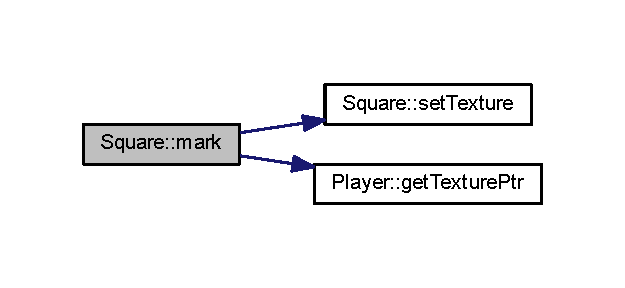
\includegraphics[width=300pt]{class_square_ab425c2f7271014c9d01eff4b0e053b31_cgraph}
\end{center}
\end{figure}




Here is the caller graph for this function\+:\nopagebreak
\begin{figure}[H]
\begin{center}
\leavevmode
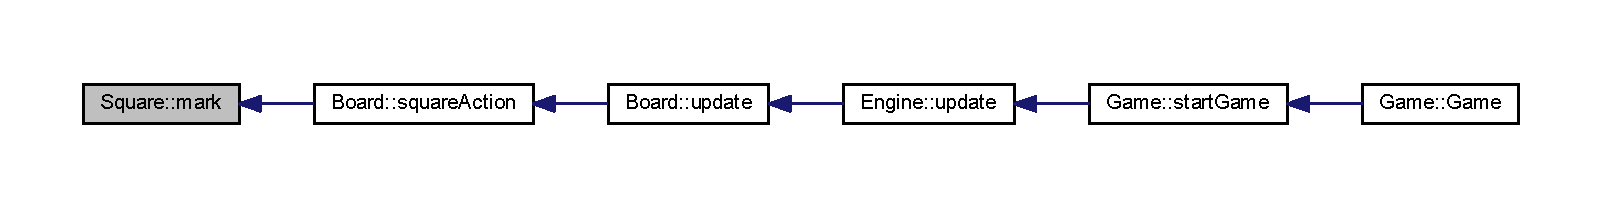
\includegraphics[width=350pt]{class_square_ab425c2f7271014c9d01eff4b0e053b31_icgraph}
\end{center}
\end{figure}


\hypertarget{class_square_a719a5dee91eaa87a7128061193388648}{}\index{Square@{Square}!set\+Position@{set\+Position}}
\index{set\+Position@{set\+Position}!Square@{Square}}
\subsubsection[{set\+Position}]{\setlength{\rightskip}{0pt plus 5cm}void Square\+::set\+Position (
\begin{DoxyParamCaption}
\item[{float}]{x, }
\item[{float}]{y}
\end{DoxyParamCaption}
)\hspace{0.3cm}{\ttfamily [private]}, {\ttfamily [virtual]}}\label{class_square_a719a5dee91eaa87a7128061193388648}


Sets position of sf\+::\+Rectangle\+Shape square. 



Here is the caller graph for this function\+:\nopagebreak
\begin{figure}[H]
\begin{center}
\leavevmode
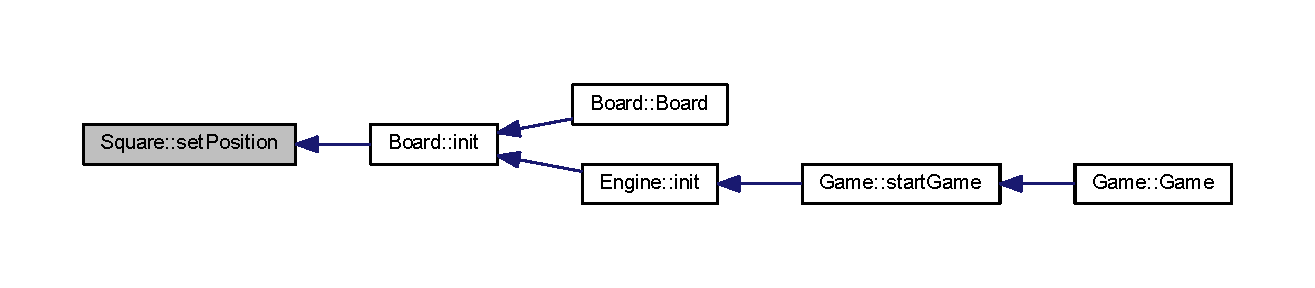
\includegraphics[width=350pt]{class_square_a719a5dee91eaa87a7128061193388648_icgraph}
\end{center}
\end{figure}


\hypertarget{class_square_ad62196a5af085b2cd38df1cc698226c8}{}\index{Square@{Square}!set\+Texture@{set\+Texture}}
\index{set\+Texture@{set\+Texture}!Square@{Square}}
\subsubsection[{set\+Texture}]{\setlength{\rightskip}{0pt plus 5cm}void Square\+::set\+Texture (
\begin{DoxyParamCaption}
\item[{sf\+::\+Texture $\ast$}]{texture}
\end{DoxyParamCaption}
)\hspace{0.3cm}{\ttfamily [private]}}\label{class_square_ad62196a5af085b2cd38df1cc698226c8}


This is function used by current class to set \hyperlink{class_square}{Square(and sf\+::\+Rectangle\+Shape)} current texture. 



Here is the caller graph for this function\+:\nopagebreak
\begin{figure}[H]
\begin{center}
\leavevmode
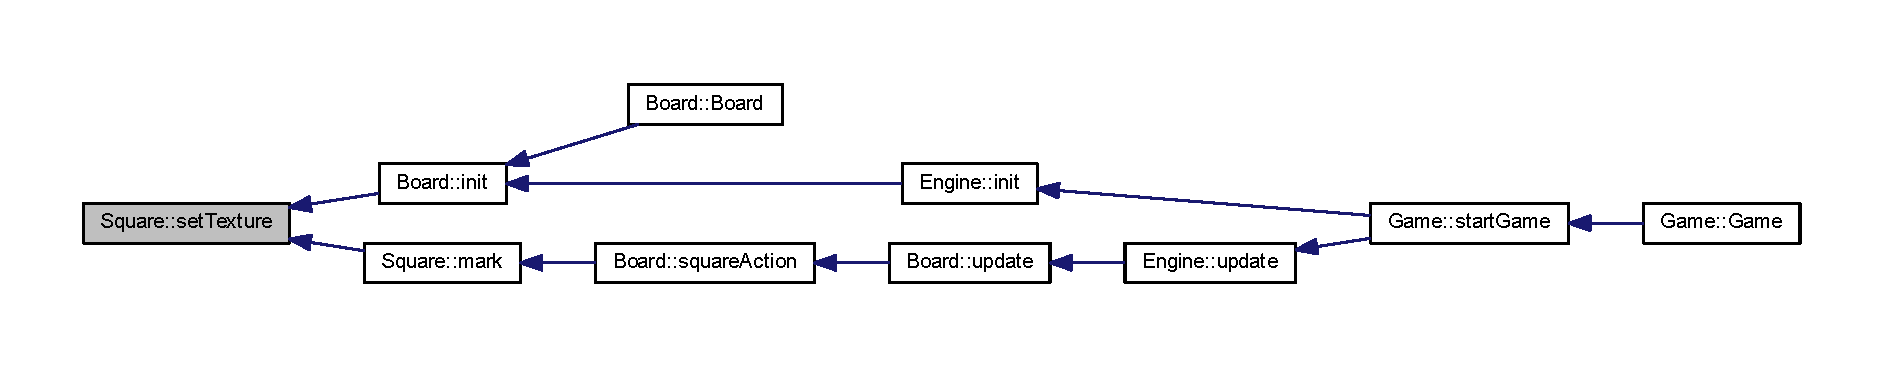
\includegraphics[width=350pt]{class_square_ad62196a5af085b2cd38df1cc698226c8_icgraph}
\end{center}
\end{figure}




\subsection{Friends And Related Function Documentation}
\hypertarget{class_square_a12525b6ed7c8186be0bee5cf78e2a49c}{}\index{Square@{Square}!Board@{Board}}
\index{Board@{Board}!Square@{Square}}
\subsubsection[{Board}]{\setlength{\rightskip}{0pt plus 5cm}friend class {\bf Board}\hspace{0.3cm}{\ttfamily [friend]}}\label{class_square_a12525b6ed7c8186be0bee5cf78e2a49c}


\subsection{Member Data Documentation}
\hypertarget{class_square_a1304492dc99a6af1f0bf2ab24d97520a}{}\index{Square@{Square}!marked\+\_\+by@{marked\+\_\+by}}
\index{marked\+\_\+by@{marked\+\_\+by}!Square@{Square}}
\subsubsection[{marked\+\_\+by}]{\setlength{\rightskip}{0pt plus 5cm}{\bf Player}$\ast$ Square\+::marked\+\_\+by\hspace{0.3cm}{\ttfamily [private]}}\label{class_square_a1304492dc99a6af1f0bf2ab24d97520a}


variable used to save who marked current \hyperlink{class_square}{Square} 

\hypertarget{class_square_a973d093bc18730c9ad2e74f9866af996}{}\index{Square@{Square}!square@{square}}
\index{square@{square}!Square@{Square}}
\subsubsection[{square}]{\setlength{\rightskip}{0pt plus 5cm}sf\+::\+Rectangle\+Shape Square\+::square\hspace{0.3cm}{\ttfamily [private]}}\label{class_square_a973d093bc18730c9ad2e74f9866af996}


Shape from S\+F\+M\+L class. The whole class may inheritance form this class. 

\hypertarget{class_square_a9bd6a0eca56aa3075227f56ee54d7808}{}\index{Square@{Square}!texture@{texture}}
\index{texture@{texture}!Square@{Square}}
\subsubsection[{texture}]{\setlength{\rightskip}{0pt plus 5cm}sf\+::\+Texture$\ast$ Square\+::texture\hspace{0.3cm}{\ttfamily [private]}}\label{class_square_a9bd6a0eca56aa3075227f56ee54d7808}


Pointer to current \hyperlink{class_square}{Square( sf\+::\+Rectangle\+Shape square )} texture. Marking change texture to player texture; this is going to be remade. 



The documentation for this class was generated from the following files\+:\begin{DoxyCompactItemize}
\item 
\hyperlink{_square_8h}{Square.\+h}\item 
\hyperlink{_square_8cpp}{Square.\+cpp}\end{DoxyCompactItemize}

\chapter{File Documentation}
\hypertarget{_board_8cpp}{}\section{Board.\+cpp File Reference}
\label{_board_8cpp}\index{Board.\+cpp@{Board.\+cpp}}
{\ttfamily \#include \char`\"{}Board.\+h\char`\"{}}\\*
{\ttfamily \#include $<$iostream$>$}\\*
{\ttfamily \#include $<$assert.\+h$>$}\\*
Include dependency graph for Board.\+cpp\+:\nopagebreak
\begin{figure}[H]
\begin{center}
\leavevmode
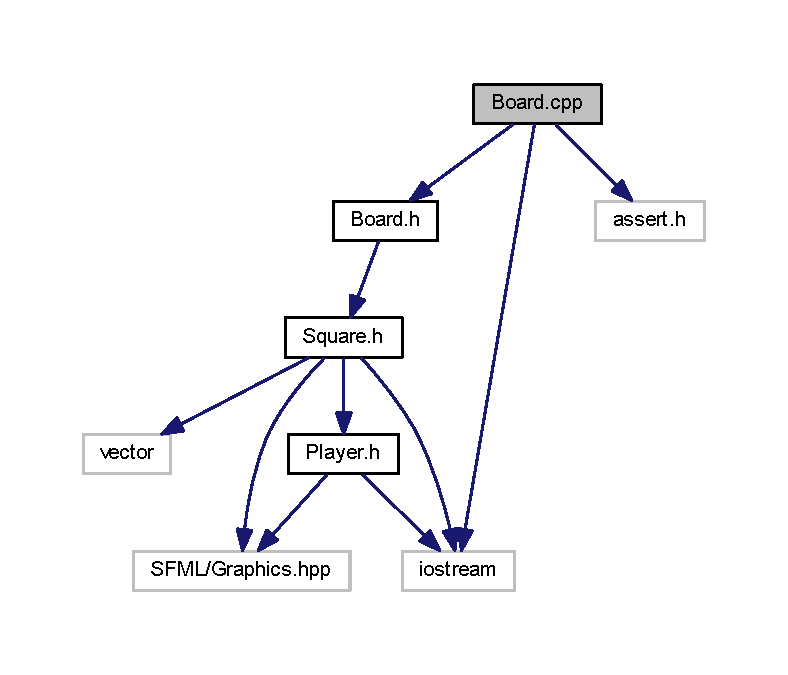
\includegraphics[width=350pt]{_board_8cpp__incl}
\end{center}
\end{figure}

\hypertarget{_board_8h}{}\section{Board.\+h File Reference}
\label{_board_8h}\index{Board.\+h@{Board.\+h}}
{\ttfamily \#include \char`\"{}Square.\+h\char`\"{}}\\*
Include dependency graph for Board.\+h\+:\nopagebreak
\begin{figure}[H]
\begin{center}
\leavevmode
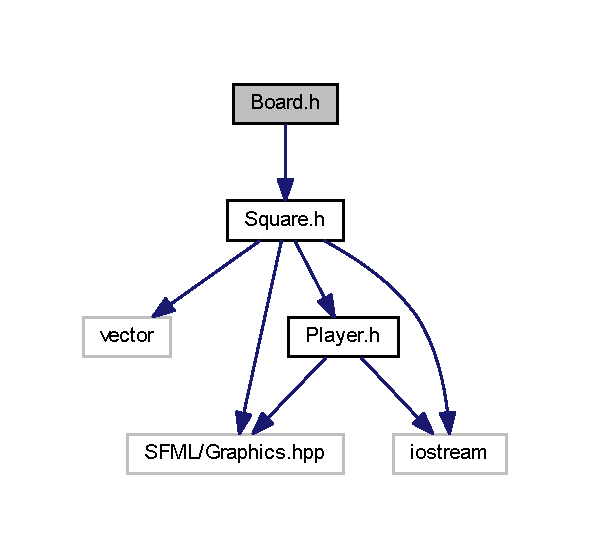
\includegraphics[width=283pt]{_board_8h__incl}
\end{center}
\end{figure}
This graph shows which files directly or indirectly include this file\+:\nopagebreak
\begin{figure}[H]
\begin{center}
\leavevmode
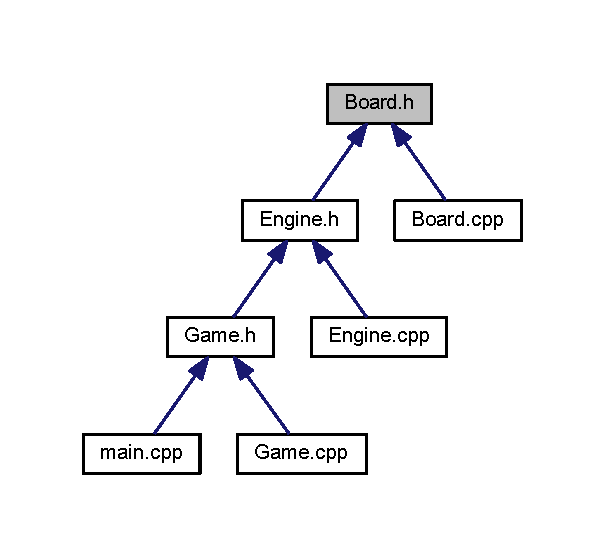
\includegraphics[width=291pt]{_board_8h__dep__incl}
\end{center}
\end{figure}
\subsection*{Classes}
\begin{DoxyCompactItemize}
\item 
class \hyperlink{class_board}{Board}
\begin{DoxyCompactList}\small\item\em \hyperlink{class_engine}{Engine} class. Class which manage main loop of game, reads keyboard events, update physics. This class will menage menu and settings. \end{DoxyCompactList}\end{DoxyCompactItemize}
\subsection*{Macros}
\begin{DoxyCompactItemize}
\item 
\#define \hyperlink{_board_8h_afb52a17f9d1f5595f2ae2cfc9abb49b4}{I\+N\+\_\+\+A\+\_\+\+R\+O\+W\+\_\+\+T\+O\+\_\+\+W\+I\+N}~5
\item 
\#define \hyperlink{_board_8h_aed89bd71aee8be823e8a20ec4e093c1e}{H\+E\+I\+G\+H\+T}~20
\item 
\#define \hyperlink{_board_8h_a241aeeb764887ae5e3de58b98f04b16d}{W\+I\+D\+T\+H}~30
\end{DoxyCompactItemize}


\subsection{Macro Definition Documentation}
\hypertarget{_board_8h_aed89bd71aee8be823e8a20ec4e093c1e}{}\index{Board.\+h@{Board.\+h}!H\+E\+I\+G\+H\+T@{H\+E\+I\+G\+H\+T}}
\index{H\+E\+I\+G\+H\+T@{H\+E\+I\+G\+H\+T}!Board.\+h@{Board.\+h}}
\subsubsection[{H\+E\+I\+G\+H\+T}]{\setlength{\rightskip}{0pt plus 5cm}\#define H\+E\+I\+G\+H\+T~20}\label{_board_8h_aed89bd71aee8be823e8a20ec4e093c1e}
\hypertarget{_board_8h_afb52a17f9d1f5595f2ae2cfc9abb49b4}{}\index{Board.\+h@{Board.\+h}!I\+N\+\_\+\+A\+\_\+\+R\+O\+W\+\_\+\+T\+O\+\_\+\+W\+I\+N@{I\+N\+\_\+\+A\+\_\+\+R\+O\+W\+\_\+\+T\+O\+\_\+\+W\+I\+N}}
\index{I\+N\+\_\+\+A\+\_\+\+R\+O\+W\+\_\+\+T\+O\+\_\+\+W\+I\+N@{I\+N\+\_\+\+A\+\_\+\+R\+O\+W\+\_\+\+T\+O\+\_\+\+W\+I\+N}!Board.\+h@{Board.\+h}}
\subsubsection[{I\+N\+\_\+\+A\+\_\+\+R\+O\+W\+\_\+\+T\+O\+\_\+\+W\+I\+N}]{\setlength{\rightskip}{0pt plus 5cm}\#define I\+N\+\_\+\+A\+\_\+\+R\+O\+W\+\_\+\+T\+O\+\_\+\+W\+I\+N~5}\label{_board_8h_afb52a17f9d1f5595f2ae2cfc9abb49b4}
\hypertarget{_board_8h_a241aeeb764887ae5e3de58b98f04b16d}{}\index{Board.\+h@{Board.\+h}!W\+I\+D\+T\+H@{W\+I\+D\+T\+H}}
\index{W\+I\+D\+T\+H@{W\+I\+D\+T\+H}!Board.\+h@{Board.\+h}}
\subsubsection[{W\+I\+D\+T\+H}]{\setlength{\rightskip}{0pt plus 5cm}\#define W\+I\+D\+T\+H~30}\label{_board_8h_a241aeeb764887ae5e3de58b98f04b16d}

\hypertarget{_engine_8cpp}{}\section{Engine.\+cpp File Reference}
\label{_engine_8cpp}\index{Engine.\+cpp@{Engine.\+cpp}}
{\ttfamily \#include \char`\"{}Engine.\+h\char`\"{}}\\*
{\ttfamily \#include $<$iostream$>$}\\*
Include dependency graph for Engine.\+cpp\+:\nopagebreak
\begin{figure}[H]
\begin{center}
\leavevmode
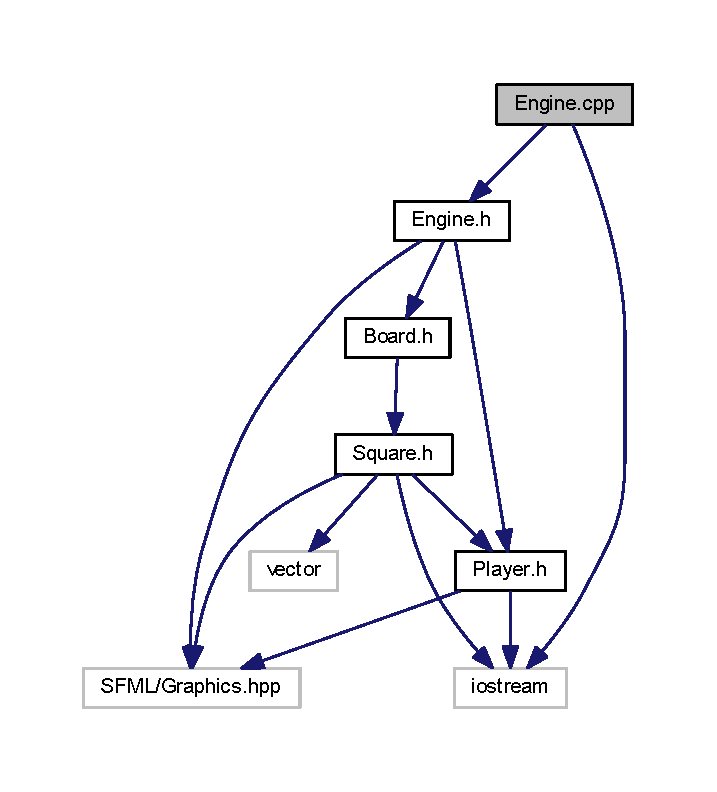
\includegraphics[width=344pt]{_engine_8cpp__incl}
\end{center}
\end{figure}
\subsection*{Macros}
\begin{DoxyCompactItemize}
\item 
\#define \hyperlink{_engine_8cpp_aed89bd71aee8be823e8a20ec4e093c1e}{H\+E\+I\+G\+H\+T}~20
\item 
\#define \hyperlink{_engine_8cpp_a241aeeb764887ae5e3de58b98f04b16d}{W\+I\+D\+T\+H}~30
\end{DoxyCompactItemize}
\subsection*{Functions}
\begin{DoxyCompactItemize}
\item 
bool \hyperlink{_engine_8cpp_a569a3713058cac3a550a9c77a55b96ea}{full\+Board\+Check} (sf\+::\+Render\+Window \&window)
\end{DoxyCompactItemize}


\subsection{Macro Definition Documentation}
\hypertarget{_engine_8cpp_aed89bd71aee8be823e8a20ec4e093c1e}{}\index{Engine.\+cpp@{Engine.\+cpp}!H\+E\+I\+G\+H\+T@{H\+E\+I\+G\+H\+T}}
\index{H\+E\+I\+G\+H\+T@{H\+E\+I\+G\+H\+T}!Engine.\+cpp@{Engine.\+cpp}}
\subsubsection[{H\+E\+I\+G\+H\+T}]{\setlength{\rightskip}{0pt plus 5cm}\#define H\+E\+I\+G\+H\+T~20}\label{_engine_8cpp_aed89bd71aee8be823e8a20ec4e093c1e}
\hypertarget{_engine_8cpp_a241aeeb764887ae5e3de58b98f04b16d}{}\index{Engine.\+cpp@{Engine.\+cpp}!W\+I\+D\+T\+H@{W\+I\+D\+T\+H}}
\index{W\+I\+D\+T\+H@{W\+I\+D\+T\+H}!Engine.\+cpp@{Engine.\+cpp}}
\subsubsection[{W\+I\+D\+T\+H}]{\setlength{\rightskip}{0pt plus 5cm}\#define W\+I\+D\+T\+H~30}\label{_engine_8cpp_a241aeeb764887ae5e3de58b98f04b16d}


\subsection{Function Documentation}
\hypertarget{_engine_8cpp_a569a3713058cac3a550a9c77a55b96ea}{}\index{Engine.\+cpp@{Engine.\+cpp}!full\+Board\+Check@{full\+Board\+Check}}
\index{full\+Board\+Check@{full\+Board\+Check}!Engine.\+cpp@{Engine.\+cpp}}
\subsubsection[{full\+Board\+Check}]{\setlength{\rightskip}{0pt plus 5cm}bool full\+Board\+Check (
\begin{DoxyParamCaption}
\item[{sf\+::\+Render\+Window \&}]{window}
\end{DoxyParamCaption}
)}\label{_engine_8cpp_a569a3713058cac3a550a9c77a55b96ea}

\hypertarget{_engine_8cpp_8cpp}{}\section{Engine.\+cpp.\+cpp File Reference}
\label{_engine_8cpp_8cpp}\index{Engine.\+cpp.\+cpp@{Engine.\+cpp.\+cpp}}
{\ttfamily \#include \char`\"{}Engine.\+cpp.\+h\char`\"{}}\\*
Include dependency graph for Engine.\+cpp.\+cpp\+:\nopagebreak
\begin{figure}[H]
\begin{center}
\leavevmode
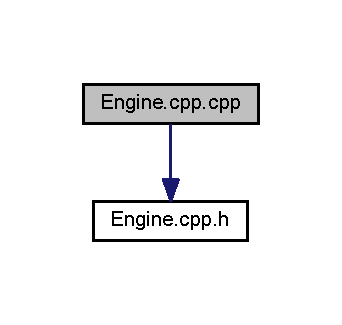
\includegraphics[width=164pt]{_engine_8cpp_8cpp__incl}
\end{center}
\end{figure}
\subsection*{Functions}
\begin{DoxyCompactItemize}
\item 
\hyperlink{class_engine}{Engine} cpp\+::\+Engine \hyperlink{_engine_8cpp_8cpp_a9840bdd08dfba872438b3dbcab02e510}{cpp} ()
\end{DoxyCompactItemize}


\subsection{Function Documentation}
\hypertarget{_engine_8cpp_8cpp_a9840bdd08dfba872438b3dbcab02e510}{}\index{Engine.\+cpp.\+cpp@{Engine.\+cpp.\+cpp}!cpp@{cpp}}
\index{cpp@{cpp}!Engine.\+cpp.\+cpp@{Engine.\+cpp.\+cpp}}
\subsubsection[{cpp}]{\setlength{\rightskip}{0pt plus 5cm}{\bf Engine} cpp\+::$\sim$\+Engine cpp (
\begin{DoxyParamCaption}
{}
\end{DoxyParamCaption}
)}\label{_engine_8cpp_8cpp_a9840bdd08dfba872438b3dbcab02e510}

\hypertarget{_engine_8cpp_8h}{}\section{Engine.\+cpp.\+h File Reference}
\label{_engine_8cpp_8h}\index{Engine.\+cpp.\+h@{Engine.\+cpp.\+h}}
This graph shows which files directly or indirectly include this file\+:\nopagebreak
\begin{figure}[H]
\begin{center}
\leavevmode
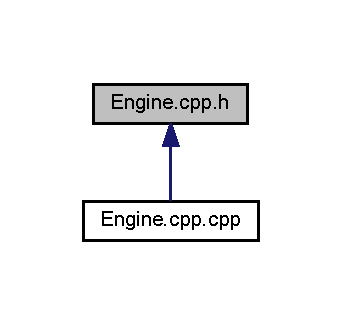
\includegraphics[width=164pt]{_engine_8cpp_8h__dep__incl}
\end{center}
\end{figure}
\subsection*{Classes}
\begin{DoxyCompactItemize}
\item 
class \hyperlink{class_engine_1_1cpp}{Engine\+::cpp}
\end{DoxyCompactItemize}

\hypertarget{_engine_8h}{}\section{Engine.\+h File Reference}
\label{_engine_8h}\index{Engine.\+h@{Engine.\+h}}
{\ttfamily \#include $<$S\+F\+M\+L/\+Graphics.\+hpp$>$}\\*
{\ttfamily \#include $<$Board.\+h$>$}\\*
{\ttfamily \#include \char`\"{}Player.\+h\char`\"{}}\\*
Include dependency graph for Engine.\+h\+:\nopagebreak
\begin{figure}[H]
\begin{center}
\leavevmode
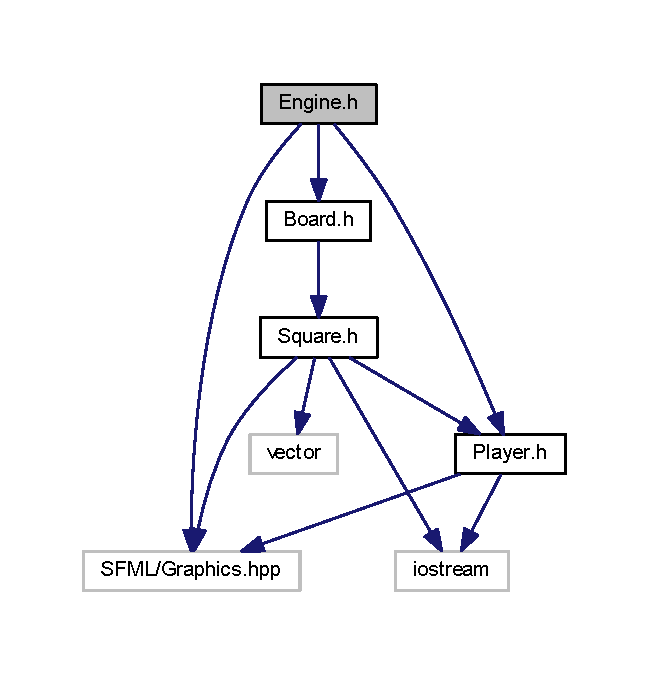
\includegraphics[width=312pt]{_engine_8h__incl}
\end{center}
\end{figure}
This graph shows which files directly or indirectly include this file\+:\nopagebreak
\begin{figure}[H]
\begin{center}
\leavevmode
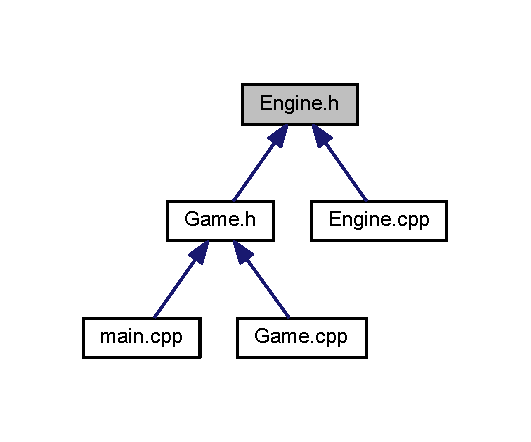
\includegraphics[width=255pt]{_engine_8h__dep__incl}
\end{center}
\end{figure}
\subsection*{Classes}
\begin{DoxyCompactItemize}
\item 
class \hyperlink{class_engine}{Engine}
\begin{DoxyCompactList}\small\item\em \hyperlink{class_engine}{Engine} class. Class which manage main loop of game, reads keyboard events, update physics. This class will menage menu and settings. \end{DoxyCompactList}\end{DoxyCompactItemize}

\hypertarget{_game_8cpp}{}\section{Game.\+cpp File Reference}
\label{_game_8cpp}\index{Game.\+cpp@{Game.\+cpp}}
{\ttfamily \#include \char`\"{}Game.\+h\char`\"{}}\\*
Include dependency graph for Game.\+cpp\+:\nopagebreak
\begin{figure}[H]
\begin{center}
\leavevmode
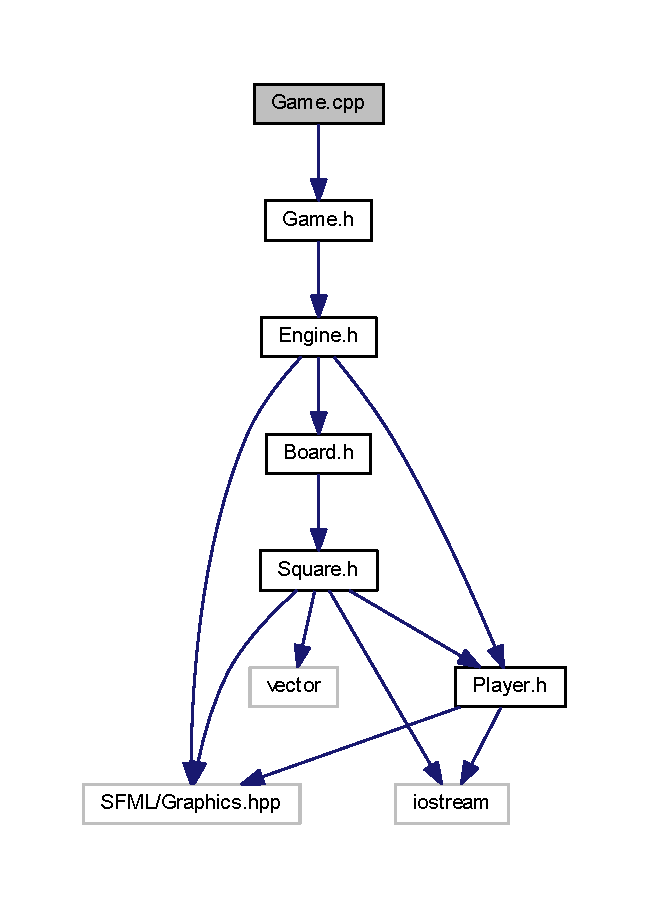
\includegraphics[width=312pt]{_game_8cpp__incl}
\end{center}
\end{figure}

\hypertarget{_game_8h}{}\section{Game.\+h File Reference}
\label{_game_8h}\index{Game.\+h@{Game.\+h}}
{\ttfamily \#include \char`\"{}Engine.\+h\char`\"{}}\\*
Include dependency graph for Game.\+h\+:\nopagebreak
\begin{figure}[H]
\begin{center}
\leavevmode
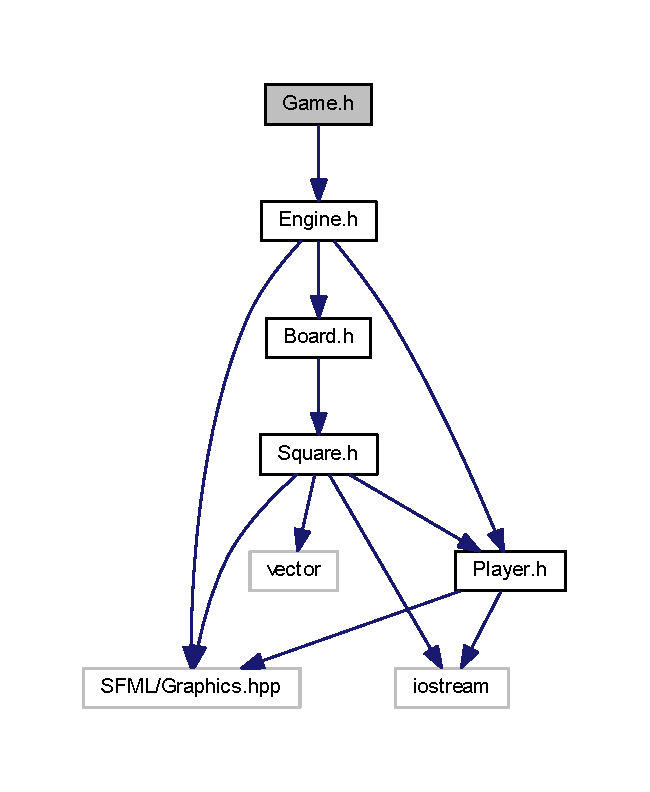
\includegraphics[width=312pt]{_game_8h__incl}
\end{center}
\end{figure}
This graph shows which files directly or indirectly include this file\+:\nopagebreak
\begin{figure}[H]
\begin{center}
\leavevmode
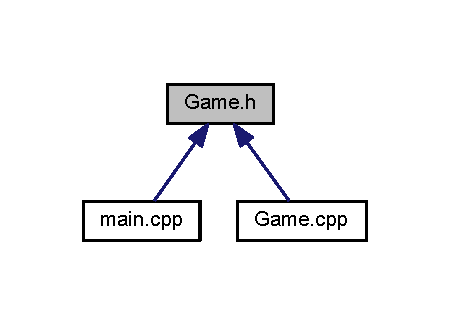
\includegraphics[width=216pt]{_game_8h__dep__incl}
\end{center}
\end{figure}
\subsection*{Classes}
\begin{DoxyCompactItemize}
\item 
class \hyperlink{class_game}{Game}
\begin{DoxyCompactList}\small\item\em \hyperlink{class_game}{Game} main class. Class which is used run engine. This class will menage menu and settings. \end{DoxyCompactList}\end{DoxyCompactItemize}

\hypertarget{main_8cpp}{}\section{main.\+cpp File Reference}
\label{main_8cpp}\index{main.\+cpp@{main.\+cpp}}


Main file of the program.  


{\ttfamily \#include $<$iostream$>$}\\*
\subsection*{Functions}
\begin{DoxyCompactItemize}
\item 
\hypertarget{main_8cpp_ae66f6b31b5ad750f1fe042a706a4e3d4}{}int {\bfseries main} ()\label{main_8cpp_ae66f6b31b5ad750f1fe042a706a4e3d4}

\end{DoxyCompactItemize}


\subsection{Detailed Description}
Main file of the program. 

\begin{DoxyNote}{Note}
with gh-\/pages
\end{DoxyNote}
\begin{DoxyAuthor}{Author}
(last to touch it) 
\end{DoxyAuthor}
\begin{DoxyParagraph}{Author}
bv Foto
\end{DoxyParagraph}


\begin{DoxyVersion}{Version}

\end{DoxyVersion}
\begin{DoxyParagraph}{Revision}
0.\+01 
\end{DoxyParagraph}


\begin{DoxyDate}{Date}

\end{DoxyDate}
\begin{DoxyParagraph}{Date}
2016/03/13 21\+:44\+:00 
\end{DoxyParagraph}


Contact\+: \href{mailto:fotoblysk@fejm.pl}{\tt fotoblysk@fejm.\+pl}

Created on\+: Sun Mar 13 21\+:44\+:00 2016

\begin{DoxyParagraph}{Id}
Cross-\/and-\/circle-\/game,v 0.\+01 21\+:44\+:00 bv Exp Foto
\end{DoxyParagraph}

\hypertarget{_player_8cpp}{}\section{Player.\+cpp File Reference}
\label{_player_8cpp}\index{Player.\+cpp@{Player.\+cpp}}
{\ttfamily \#include \char`\"{}Player.\+h\char`\"{}}\\*
Include dependency graph for Player.\+cpp\+:\nopagebreak
\begin{figure}[H]
\begin{center}
\leavevmode
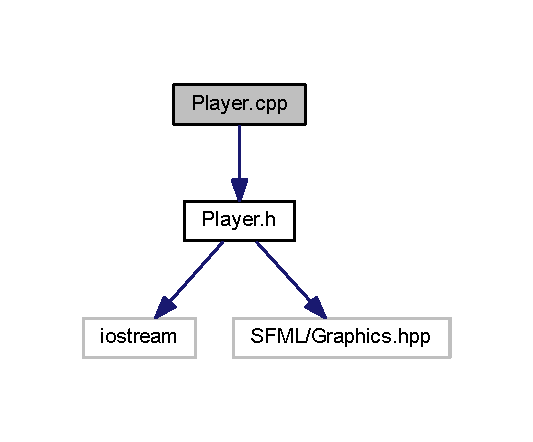
\includegraphics[width=256pt]{_player_8cpp__incl}
\end{center}
\end{figure}

\hypertarget{_player_8h}{}\section{Player.\+h File Reference}
\label{_player_8h}\index{Player.\+h@{Player.\+h}}
{\ttfamily \#include $<$iostream$>$}\\*
{\ttfamily \#include $<$S\+F\+M\+L/\+Graphics.\+hpp$>$}\\*
Include dependency graph for Player.\+h\+:\nopagebreak
\begin{figure}[H]
\begin{center}
\leavevmode
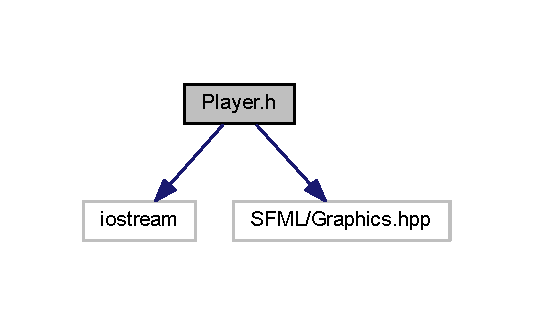
\includegraphics[width=256pt]{_player_8h__incl}
\end{center}
\end{figure}
This graph shows which files directly or indirectly include this file\+:\nopagebreak
\begin{figure}[H]
\begin{center}
\leavevmode
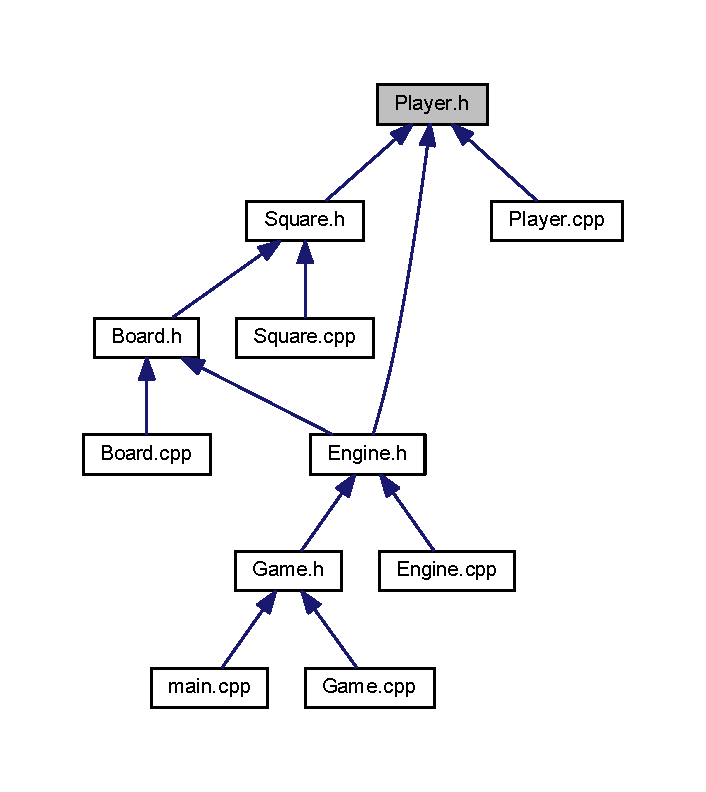
\includegraphics[width=339pt]{_player_8h__dep__incl}
\end{center}
\end{figure}
\subsection*{Classes}
\begin{DoxyCompactItemize}
\item 
class \hyperlink{class_player}{Player}
\begin{DoxyCompactList}\small\item\em \hyperlink{class_player}{Player} class -\/ pointers to player have a lot of usage in program. All Squares have pointer to player which were marked by pointers to players are also used by \hyperlink{class_engine}{Engine} class to set whose turn is now. \end{DoxyCompactList}\end{DoxyCompactItemize}
\subsection*{Macros}
\begin{DoxyCompactItemize}
\item 
\#define \hyperlink{_player_8h_af1206b4d3bda8c4c8c9257f369a9e9e1}{D\+E\+B\+U\+G\+\_\+\+M\+S\+G}(str)~do \{ std\+::cout $<$$<$ str;\} while( false )
\end{DoxyCompactItemize}


\subsection{Macro Definition Documentation}
\hypertarget{_player_8h_af1206b4d3bda8c4c8c9257f369a9e9e1}{}\index{Player.\+h@{Player.\+h}!D\+E\+B\+U\+G\+\_\+\+M\+S\+G@{D\+E\+B\+U\+G\+\_\+\+M\+S\+G}}
\index{D\+E\+B\+U\+G\+\_\+\+M\+S\+G@{D\+E\+B\+U\+G\+\_\+\+M\+S\+G}!Player.\+h@{Player.\+h}}
\subsubsection[{D\+E\+B\+U\+G\+\_\+\+M\+S\+G}]{\setlength{\rightskip}{0pt plus 5cm}\#define D\+E\+B\+U\+G\+\_\+\+M\+S\+G(
\begin{DoxyParamCaption}
\item[{}]{str}
\end{DoxyParamCaption}
)~do \{ std\+::cout $<$$<$ str;\} while( false )}\label{_player_8h_af1206b4d3bda8c4c8c9257f369a9e9e1}

\hypertarget{_r_e_a_d_m_e_8md}{}\section{R\+E\+A\+D\+M\+E.\+md File Reference}
\label{_r_e_a_d_m_e_8md}\index{R\+E\+A\+D\+M\+E.\+md@{R\+E\+A\+D\+M\+E.\+md}}

\hypertarget{_square_8cpp}{}\section{Square.\+cpp File Reference}
\label{_square_8cpp}\index{Square.\+cpp@{Square.\+cpp}}
{\ttfamily \#include \char`\"{}Square.\+h\char`\"{}}\\*
{\ttfamily \#include $<$iostream$>$}\\*
Include dependency graph for Square.\+cpp\+:\nopagebreak
\begin{figure}[H]
\begin{center}
\leavevmode
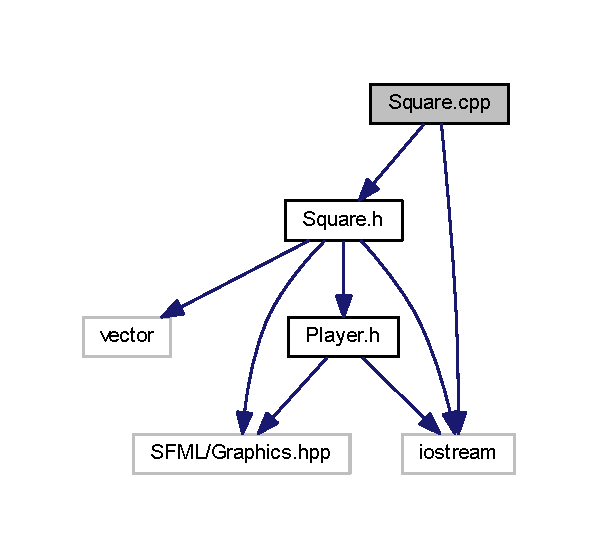
\includegraphics[width=287pt]{_square_8cpp__incl}
\end{center}
\end{figure}

\hypertarget{_square_8h}{}\section{Square.\+h File Reference}
\label{_square_8h}\index{Square.\+h@{Square.\+h}}
{\ttfamily \#include $<$vector$>$}\\*
{\ttfamily \#include $<$S\+F\+M\+L/\+Graphics.\+hpp$>$}\\*
{\ttfamily \#include $<$iostream$>$}\\*
{\ttfamily \#include \char`\"{}Player.\+h\char`\"{}}\\*
Include dependency graph for Square.\+h\+:\nopagebreak
\begin{figure}[H]
\begin{center}
\leavevmode
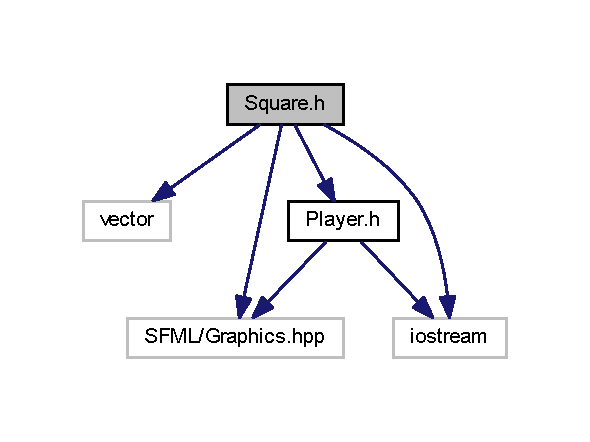
\includegraphics[width=283pt]{_square_8h__incl}
\end{center}
\end{figure}
This graph shows which files directly or indirectly include this file\+:\nopagebreak
\begin{figure}[H]
\begin{center}
\leavevmode
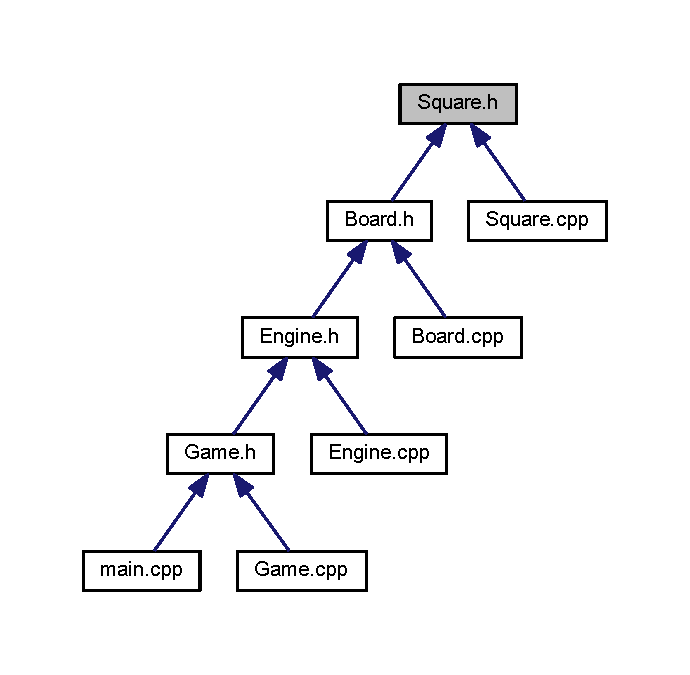
\includegraphics[width=331pt]{_square_8h__dep__incl}
\end{center}
\end{figure}
\subsection*{Classes}
\begin{DoxyCompactItemize}
\item 
class \hyperlink{class_square}{Square}
\begin{DoxyCompactList}\small\item\em \hyperlink{class_square}{Square} class. Class which is used to build board this class may be remade to inheritance from sf\+::\+Rectangle\+Shape. \end{DoxyCompactList}\end{DoxyCompactItemize}
\subsection*{Macros}
\begin{DoxyCompactItemize}
\item 
\#define \hyperlink{_square_8h_aa465c0206c08c9cde6075c2afb1c8bc8}{S\+Q\+U\+A\+R\+E\+\_\+\+S\+I\+Z\+E}~50
\item 
\#define \hyperlink{_square_8h_af1206b4d3bda8c4c8c9257f369a9e9e1}{D\+E\+B\+U\+G\+\_\+\+M\+S\+G}(str)~do \{ std\+::cout $<$$<$ str;\} while( false )
\end{DoxyCompactItemize}


\subsection{Macro Definition Documentation}
\hypertarget{_square_8h_af1206b4d3bda8c4c8c9257f369a9e9e1}{}\index{Square.\+h@{Square.\+h}!D\+E\+B\+U\+G\+\_\+\+M\+S\+G@{D\+E\+B\+U\+G\+\_\+\+M\+S\+G}}
\index{D\+E\+B\+U\+G\+\_\+\+M\+S\+G@{D\+E\+B\+U\+G\+\_\+\+M\+S\+G}!Square.\+h@{Square.\+h}}
\subsubsection[{D\+E\+B\+U\+G\+\_\+\+M\+S\+G}]{\setlength{\rightskip}{0pt plus 5cm}\#define D\+E\+B\+U\+G\+\_\+\+M\+S\+G(
\begin{DoxyParamCaption}
\item[{}]{str}
\end{DoxyParamCaption}
)~do \{ std\+::cout $<$$<$ str;\} while( false )}\label{_square_8h_af1206b4d3bda8c4c8c9257f369a9e9e1}
\hypertarget{_square_8h_aa465c0206c08c9cde6075c2afb1c8bc8}{}\index{Square.\+h@{Square.\+h}!S\+Q\+U\+A\+R\+E\+\_\+\+S\+I\+Z\+E@{S\+Q\+U\+A\+R\+E\+\_\+\+S\+I\+Z\+E}}
\index{S\+Q\+U\+A\+R\+E\+\_\+\+S\+I\+Z\+E@{S\+Q\+U\+A\+R\+E\+\_\+\+S\+I\+Z\+E}!Square.\+h@{Square.\+h}}
\subsubsection[{S\+Q\+U\+A\+R\+E\+\_\+\+S\+I\+Z\+E}]{\setlength{\rightskip}{0pt plus 5cm}\#define S\+Q\+U\+A\+R\+E\+\_\+\+S\+I\+Z\+E~50}\label{_square_8h_aa465c0206c08c9cde6075c2afb1c8bc8}

%--- End generated contents ---

% Index
\backmatter
\newpage
\phantomsection
\clearemptydoublepage
\addcontentsline{toc}{chapter}{Index}
\printindex

\end{document}
